\documentclass{paper}\usepackage{graphicx}
\usepackage{hyperref}
\usepackage[capitalise, nameinlink, sort]{cleveref}
\usepackage{booktabs}
\usepackage{microtype}
\usepackage{subcaption}
\usepackage{tikz}
\usepackage{tabularx}
\usepackage{changepage}
\usepackage{xspace}
\usepackage{amssymb}
\newcommand{\ie}{\emph{i.e.}\@\xspace}
\newcommand{\eg}{\emph{e.g.}\@\xspace}
\makeatletter
\newcommand*{\etc}{\@ifnextchar{.}{etc}{etc.\@\xspace}}
\makeatother
\newcommand{\etal}{\emph{et al.}\@\xspace}
\usepackage[section]{placeins}
\usepackage{listings}
\usepackage{graphicx}
\usepackage[capitalise, nameinlink, sort]{cleveref}
\usepackage{booktabs}
\usepackage{microtype}
%\usepackage{subcaption}
\usepackage{tikz}
\usepackage{tabularx}
\usepackage{changepage}
\usepackage{xspace}
\usepackage{amssymb}
\usepackage{multicol}
%\usepackage{subfigure}

%%%%% fix for caption being too close to table
\usepackage{caption}
\captionsetup[table]{skip=5pt}
%%%% end fix

%\usepackage{pgfplotstable}
\usepackage{makecell}

\renewcommand\UrlFont{\color{blue}\rmfamily}

\makeatletter
\newcommand\footnoteref[1]{\protected@xdef\@thefnmark{\ref{#1}}\@footnotemark}
\makeatother

%\usepackage{todonotes}
\usepackage[disable]{todonotes}
\newcommand{\ptcom}[1]{\todo[inline, color=green!40]{PT: #1}}
\newcommand{\bacom}[1]{\todo[inline, color=blue!40]{BA: #1}}
\newcommand{\rmcom}[1]{\todo[inline, color=red!40]{RM: #1}}

\definecolor{safelightblue}{rgb}{0.65098, 0.807843, 0.890196}
\definecolor{safelightgrey}{rgb}{0.7, 0.7, 0.7}

\tikzset{vertex/.style={draw, circle, inner sep=0pt, minimum size=0.5cm, font=\small\bfseries}}
\tikzset{vertexc1/.style={vertex, fill=safelightblue}}
\tikzset{edge/.style={color=safelightgrey}}
\tikzset{bedge/.style={ultra thick}}


\usepackage[capitalise, nameinlink, sort]{cleveref}
\crefname{lstlisting}{Listing}{Listings}
\Crefname{lstlisting}{Listing}{Listings}

\usepackage{listings}

\definecolor{solarized@base03}{HTML}{002B36}
\definecolor{solarized@base02}{HTML}{073642}
\definecolor{solarized@base01}{HTML}{586e75}
\definecolor{solarized@base00}{HTML}{657b83}
\definecolor{solarized@base0}{HTML}{839496}
\definecolor{solarized@base1}{HTML}{93a1a1}
\definecolor{solarized@base2}{HTML}{EEE8D5}
\definecolor{solarized@base3}{HTML}{FDF6E3}
\definecolor{solarized@yellow}{HTML}{B58900}
\definecolor{solarized@orange}{HTML}{CB4B16}
\definecolor{solarized@red}{HTML}{DC322F}
\definecolor{solarized@magenta}{HTML}{D33682}
\definecolor{solarized@violet}{HTML}{6C71C4}
\definecolor{solarized@blue}{HTML}{268BD2}
\definecolor{solarized@cyan}{HTML}{2AA198}
\definecolor{solarized@green}{HTML}{859900}

\lstnewenvironment{cpp}[1][] {
  \lstset{
  language=c++,
  basicstyle=\ttfamily\scriptsize,
  numbers=left,
  numberstyle=\tiny,
  tabsize=2,
  breaklines=true,
  escapeinside={@}{@},
  numberstyle=\tiny\color{solarized@base01},
  keywordstyle=\color{solarized@green},
  stringstyle=\color{solarized@cyan}\ttfamily,
  commentstyle=\color{solarized@base01},
  emphstyle=\color{solarized@red},
  showstringspaces=false,
  flexiblecolumns=false,
  frame=tb,
  #1
  }
}
{}
\begin{document}

% Possible Titles
% Studying the Impact of NUMA in a Managed Language Implementation
% A Study of the Impact of NUMA in Haskell
% An Evaluation of Haskell on NUMA
% Assessing the Performance of Haskell over NUMA
% Assessing the Performance of a Purely Functional Language over NUMA

\title{Improving NUMA Profiling in a Managed Language Implementation}
\author{Ruairidh MacGregor}
\matricnum{2250079m}
\date{}

\maketitle

\begin{abstract}
As the number of cores increases Non-uniform memory access (NUMA) is becoming increasingly prevalent in general purpose machines. Failing to exploit NUMA effectively increases runtime by around 10-20\%. Managed programming languages like Haskell, Java or Python don’t provide the programmer tools for controlling NUMA usage, but rather rely on the language implementation. While there is research into adapting conventional languages and Virtual Machines to NUMA, there is less work on functional languages and runtime systems. This paper surveys NUMA profiling tools at hardware, OS and language implementation levels. We systematically profile 8 benchmarks from the GHC Haskell nofib suite on a typical NUMA server (8 regions, 64 cores), using two as running examples. We demonstrate significant differences in NUMA usage between computational and data-intensive benchmarks, e.g.  local access rates of and 22\% and 30\% respectively. We show that small changes to coordination behaviour can significantly alter NUMA usage. We identify NUMA usage information not available from existing profilers and extend both the numaprof profiler, and the GHC RTS to obtain three new NUMA profiles:  OS thread allocation locality,  GC frequency (per region) and GC thread locality. The profiles suggest ways that GHC can be better adapted for NUMA architectures, e.g. adapting the centralised task distribution that creates an exceptionally heavily accessed region.
%Over the previous decades, compute hardware in server computing has radically changed. With the end of Moore's law\cite{moore1965cramming} clock speeds are no longer doubling every 18 months. This initiated the multicore revolution / emergence of multi-core servers which in turn has resulted in the widespread adoption of the processor architecture Non-uniform memory access (NUMA) to give applications good performance scalability. NUMA architectures require software to be carefully crafted in languages with explicitly memory management in order to achieve good performance scalability from the architecture. Managed programming languages such as Haskell, Java and Go suffer from a lack of language level support for writing low memory latency NUMA code as the runtime system takes on this burden. Applications can pay performance penalties (10-20\%)\cite{DBLP:conf/hpca/TangMZHHT13} if region locality is not adopted, the benefits of the architecture vanish. There has been a large volume of research dedicated to adapting Java to NUMA, however, there has been little exploration in purely functional languages such as Haskell that in itself, shows great potential for studying the performance challenges posed by NUMAs, e.g. all immutability of state leads to exceptionally high allocation rates.

%This features an in initial survey of existing NUMA profiling tools, followed by systematic profiling of Haskell programs under GHC executing on a 8 region, 64 core AMD Opteron NUMA server demonstrating the behaviour of a wide class of applications and encapsulating a number of NUMA specific metrics using existing profiling tools. Two benchmarks from the Haskell \textit{nofib} suite are used. One is \textit{prsa} - a compute intensive parallel RSA encryption algorithm and the latter, \textit{sumeuler} - a memory intensive benchmark. The work in \textit{sumeuler} features a divide \& conquer and data parallel implementations, to demonstrate the different profiles that arise from different allocation strategies. Our results demonstrate that data parallel consistently outperforms divide \& conquer, with a maximum speedup of 1.51, however, both achieve local access rates of 29.6\% \& 28.7\%, whilst \lstinline{prsa} only achieves 22.3\%. Despite, this low access locality within the same region, the most common accesses to regions are those that are at the next expected latency, directly after a local access, e.g. the second fastest expected access time.

%We extended both an existing NUMA profiler and the GHC runtime system to incorporate new metrics for NUMA. Namely, \textbf{OS thread allocation locality} was implemented in \textit{numaprof}, and, \textbf{GC frequency} (per region) and \textbf{GC thread locality} were implemented in GHC. \footnote{Extensions have been made freely available and are hosted on github.}  GHC achieves around 30\% local accesses, whilst all allocations done by pinned OS threads are 100\% local. We illuminate a centralised task distribution system which leads to many remote accesses to a single region. Thus, we show there is many potential shortcomings in GHC that require addressing.

%Finally, we propose possible strategies and fixes to help address some of the limitations discovered in the profiling. Specifically, the avoidance of centralised task creation sources and copying and distribution of data to move data as close to GHC worker threads that require it. We also give an insight into how these could be used as a basis for future work in embedding these within a managed language's runtime system to allow for dynamic adaptation of NUMA policy.
\end{abstract}

\section{Introduction}
\label{sec:intro}

Non-uniform memory access (NUMA) architectures physically partition the memory into regions, where cores share a local memory bank with some other cores and can also access remote regions via an on-chip interconnect. NUMA architectures provide a performance scalable platform for server and HPC applications. To optimise (memory access) performance for maximal performance gains requires the software implementation to be carefully crafted in a language with explicit memory management to efficiently achieve this, otherwise applications receive performance penalties. Memory allocation, layout, locality and thread placement are key in order do so.

Trade-offs must be made between these parameters: cores allocating too much remotely can lead to many (slow) remote accesses being made and possible saturation of the on-chip on-chip interconnect. In contrast, too many allocations in a single region may cause load imbalance issues and saturate the memory bus \& on-chip interconnect as too many accesses are made to a single region, hence it may be suitable to use a remote region\cite{DBLP:conf/iwmm/MajoG11}.

Developing software in languages with explicit memory management, e.g. C/C++, Rust \& Swift, that can efficiently exploit NUMA requires a substantial amount of programming effort. The implementation won't be re-usable for other NUMAs as it will be explicitly coded for the target architecture. Additionally, the tuning might be specific to certain classes of input and brittle in face of changing input characteristics. Thus, putting a strain on development times for industry and making it harder to meet important deadlines. With the increased programming effort and subsequently, lines of code, introduces far more margin for memory related issues to occur, especially if the languages is not memory safe, e.g. C\cite{DBLP:conf/asplos/Shapiro06,DBLP:conf/oopsla/Kell17}. Furthermore, Microsoft released a figure\footnote{https://msrc-blog.microsoft.com/2019/07/16/a-proactive-approach-to-more-secure-code/} which illuminates that 70\% of the bugs and security vulnerabilities found across Microsoft products were memory related. Thus, with the increased programming effort and the lack of safety granted by some languages with explicit memory management is arguably going to have a negative impact. 

Managed programming languages such as Haskell, Java \& Python offer much more reduced programming effort at the cost of added runtime overhead. Compiled managed languages feature runtime system (RTS), whilst interpreted languages use a virtual machine (VM), e.g. JVM. The goal of both RTS's \& VM's is to abstract away commonly carried out and often difficult tasks required by the programmer that aren't explicitly to do with application code, e.g. memory management. Hence, reducing development times for industry and simplifying the creation of software \cite{DBLP:conf/sac/ValkovCT18,DBLP:journals/concurrency/NystromTK08}.

Managed languages don't provide constructs that control the (1) memory allocation or (2) thread allocation (into NUMA regions). The runtime RTS/VM takes on the burden of the allocation, layout and locality of program data. Thus the programmer has lost control over adopting NUMA aware strategies for performance scalability and hence can pay performance penalties if the language implementation is not NUMA aware. Furthermore, not only does the allocation have to be handled appropriately, making the GC NUMA aware is just as important\cite{DBLP:conf/pppj/PapadakisZFK20}. Recent studies implicate that a google mail back-end and a web-search front-end on a warehouse size cluster by Google show that NUMA has an impact of 10-20\% on overall performance \cite{DBLP:conf/hpca/TangMZHHT13}.

To optimise applications executing over NUMA creates the need for informative profiling information and hence tools to capture said information. For example, the programmer must known exactly where allocations are occuring within the NUMA architecture to know if they are exploiting the architecture for maximal performance gains. Another issue one may face is load balance issues amongst regions, e.g. allocations occuring far more in one region as opposed to another. Ensuring appropriate consumption of the memory bandwidth of the system can be profiled to help detect this.

Each level of the system stack has access to different information about (NUMA) memory usage. At the lowest levels reside hardware performance counters, one above is OS level tools and finally, at the language implementation, e.g. RTS for a compiled language or VM for an interpreted language. One could profile an application written in a language with explicit memory management at the level of the source code. Common hardware counter tools are \textit{Intel VTune}, \textit{AMD $\mu$prof} and parts of Linux \textit{perf tools}. OS level tools feature parts of Linux \textit{perf tools}, \textit{numaprof}. Managed language implementation tools are not common, however, there has been work aiming to do just this in the JVM, with the creation of the \textit{PerfUtil} tool.

The Haskell\cite{marlow2010haskell} programming language is a purely functional managed programming language. GHC is currently the most popular implementation, and, as of version 8.2 features some region locality. With the main strategy being to allocate memory locally. However, there has been little systematic study about understanding the key performance challenges posed towards purely functional languages and hence is a focus of this work. Haskell is particularly useful in studying managed languages within the context of NUMA, because of the following language features: (1) Immutability of all state (2) Recursive functions (3) Lazy evaluation results in the continuous allocation and de-allocation of expressions. These 3 combined, result in Haskell achieving allocation rates exceptionally higher than other modern programming langauges such as Java. This increased memory consumption is highly advantageous for studying memory management related issues as there is more allocations occuring on the NUMA, thus substantially increasing the profiling information collected in program execution.


This work makes the following contributions:

\textbf{The systematic profiling of the impact of NUMA on parallel Haskell programs, compiled with GHC using existing compiler \& OS level memory profiling tools (\Cref{sec:eval})}: this study features an evaluation of the following metrics using a mixture of existing tools provided by the GHC heap profiler \& OS-level tools. These are all recorded on 2 \textit{nofib} Haskell benchmarks, featuring a memory intensive application, \lstinline{sumeuler}, with a divide \& conquer (DNC) approach and a data parallel method. We use the compute intensive RSA encryption algorithm, \lstinline{prsa}. Studying different classes of applications allows more knowledge with regards to the NUMA behaviour of GHC to be obtained as the applications have varying needs and exploit the architecture differently. The heap profiler in GHC is used to capture the \textit{allocation rates}. The OS-level tool \textit{numaprof} which profiles dynamic behaviour such as intra and inter region accesses. We record \textit{OS thread access locality} and \textit{OS thread NUMA distance counts}. Both of the metrics grant an insight into locality awareness by illuminating the locations of where access are coming from and where they are going to. We demonstrate significant differences in NUMA usage between computational and data-intensive benchmarks, e.g.  local access rates of and 22\% and 30\% respectively. We show that small changes to coordination behaviour can significantly alter NUMA usage.
Results show that the data parallel implementation of \lstinline{sumeuler} consistently outperforms the DNC approach, by a maximum speedup of 1.51 and a minimum of 1.13, whilst also achieving very similar local access rates, 29.6\% and 28.7\% for data parallel and DNC respectively. The \textit{OS thread locality} also illuminates that there is a specific region in which large amounts of accesses take place, common amongst all of the benchmarks. Although, the local access rates are relatively low, the OS NUMA distance counts highlight that the most common type of access is at towards regions that are at the second lowest expected access latency, with between 40-45\% of all memory accesses for each benchmark.

% However, both the GHC memory profiler and \textit{numaprof} presented shortcomings in the NUMA information that can be profiled. There is no NUMA specific information that is currently recorded in the GHC runtime system. The \textit{numaprof} tools resides at the OS level and hence does encapsulate specific GHC information on e.g. objects, GHC threads etc.

\textbf{The design, implementation, and validation of extensions to an OS-level NUMA profiler (numaprof) to record thread allocation locality (\Cref{sec:extnumaprof})}: the current version of \textit{numaprof} only gives information with regards to the number of allocations per region by OS threads and doesn't give specific data outlining the NUMA region of the thread allocating the memory. Extensions to this feature in \textit{numaprof} were carried out to record the NUMA region of the calling thread and the bytes allocated in the region, and, the output is integrated into the \textit{numaprof} UI. This allows developers to easily detect remote allocation issues across regions or highlight there can be load imbalance within the same region, e.g. the heat map gives a strong red colour in a particular region, albeit memory bandwidth measurements would confirm it or not. Such extensions have been made freely available on github\footnote{https://github.com/ruairidhm98/numaprof}. The results show that all allocations done in the benchmarks by pinned OS threads are 100\% local. The profiles identify regions with high amounts of allocated bytes and thus leading to possible explanations for the high access rates found in the \textit{OS thread access locality} profiles, as they correspond to the same region between the \textit{OS thread access locality} and \textit{OS thread allocation locality} profiles.

\textbf{The design, implementation, and validation of extensions to GHC GC profiling to cover NUMA (\Cref{sec:extghc})}: the existing GC profiler in GHC is not aware of NUMA regions. The profiler provides no information with regards to how often GC is carried out per NUMA region and does not give an insight into the location of where the objects each GC thread is processing are in the NUMA architecture. Thus, extensions to the GC were required to measure the \textit{GC frequency} (per region) and \textit{GC thread locality}. We record the \textit{GC frequency} by keeping track of the number of GCs currently being carried out per region, and the \textit{GC thread locality} simply requires obtaining the specific NUMA region of the object the GC thread is processing as well as the location of the thread itself. This allows the GHC runtime system programmer to detect shortcomings in making the garbage collector NUMA aware as it shows the locations on the NUMA architecture a GC thread is processing and the \textit{GC thread locality} allows for OS thread NUMA distance counts to be factored in the analyses. Having this information readily available in the runtime system allows for the system to use this information to be apart of a dynamic adaptation to NUMA policies or allows the developer to modify and verify the NUMA strategy in the GC. Such extensions have been made freely available on github\footnote{https://github.com/ruairidhm98/ghc}. To date, the tool is only available on Linux as it relies of the \textit{numactl} package. For generation 1 and genration 2 obejcts, the DNC implementation of \lstinline{sumeuler} shows the greatest region locality, with 86.4\% in generation 1 and 93.2\% in generation 2 objects are processed process locally. Despite this, across all benchmarks, all show poor region locality for when GC threads process static objects, with a maximum of 15.2\% of static objects being processed locally across all benchmarks, specifically for DNC.

\textbf{Strategies to better adapt GHC to exploit NUMA memory (\Cref{sec:future_work})}: this systematic study of the impact of NUMA in the Haskell programming language reveals shortcomings in how GHC's region locality features currently behave over NUMA and the new profiling information allows the current "hotspots" that require work to make more NUMA aware. To improve on these shortcomings, new strategies are outlined, featuring suggestions with regards to garbage collection, e.g. moving data closer to threads that require it; distributed memory techniques for copying data across regions. Finally, we discuss how the metrics used in this work, could be used in a system which dynamically adapts based on NUMA memory usage.

\section{Related Work}
\label{sec:background}

This section covers related work in NUMA architectures, adapting managed langauges to NUMA, Haskell and a small experiment comparing the allocation rates in Haskell to Java for a sequential \lstinline{sumeuler}.

\subsection{NUMA Architectures}
\label{sec:numa_architectures}

The technology \textit{Non-uniform memory access} (NUMA) is not new, it was developed concurrently by many companies in the 1990s such as Unisys \& Convex Computer (later known as Hewlett-Packard). NUMA architectures aim to provide performance scalability for shared memory applications running on multi-core compute machines by physically partitioning the memory of the system into regions such that each core has its own local memory which it shares with some other number of cores, and, can access remote regions via an on-chip interconnect\cite{DBLP:journals/tpds/LaRoweEH92}. 

\begin{figure}[!htb]
    \centering
    \includegraphics[width=0.75\linewidth]{Interim Report/images/numa.png}
    \caption{A NUMA architecture showing 2 regions, 4 cores per region. Cores access local memory via a bus and access remote regions via the on-chip interconnect.}
    \label{fig:my_label}
\end{figure}

Cores accessing local memory can be done so much faster (currently 1.6 to 2.2 times on the NUMA server used in this work), relative to accessing remote regions and streamed at much higher bandwidth (currently 2 times), relative to streaming from a remote region. The on-chip interconnect can be located either within the same package, between processor sockets, or both. Almost all NUMA architectures maintain cache coherence (ccNUMAs) and accomplish this via inter-processor communication between cache controllers to keep a consistent image across caches. NUMAs come in varying sizes. Clusters of small (2 or 4 region) NUMAs are already the dominant server architecture, and it is widely predicted that in the next 7 years mid-size (32 – 256 core, 2–16 region) NUMA architectures will become increasingly common in
servers and desktop/workstations.

%In contrast with NUMA is the Uniform Memory Access (UMA) architecture, which provides poorer scalability\cite{motlagh2000performance}. This is where all cores share the same bus to access memory and thus introduces a scalability bottleneck as the number of cores rises in an architecture. NUMA is currently the best mechanism to provide quick access to shared resources. As the number of cores rises above 16, shared memory architectures must opt for NUMA to grant enhanced performance scalability.

\subsection{Memory Requirements of Modern Applications}
\label{sec:memory_requirements}

Memory requirements in modern applications such as machine learning, server workloads \& big data applications are exceptionally high. The large amounts of state required to be kept track of in learning applications, internet scale services, e.g. Google server, processing of big data in \lstinline{Spark} etc requires extensive use of dynamic memory in order to process suitable information as appropriate. Thus, opting for NUMA architectures allows for performance scalability to be increased and hence execution times decreasing as a result as the number of cores rises.

Furthermore, functional programming techniques are becoming increasingly adopted due to the scalable parallelism model. Reducing shared state by making all data immutable leaves programs free of race conditions, mutexes or any other synchronisation primitive that restricts access. For example, if a program tries to insert data into an immutable data structure, the structure first needs to be cloned, e.g. a call to dynamic memory and create new data, thus increasing the allocations done by the program. In fact, this style of programming has become so increasingly popular that the Rust programming language bases its concurrency model is largely based off functional programming techniques. Other examples of where the functional paradigm has been useful is in \lstinline{MapReduce} \& \lstinline{Spark}. Specifically, the concepts of \textit{map} and \textit{reduce} are directly based off the functional concepts \textit{map} and \textit{fold}.

However, if programmers wish to make use of more scalable techniques for parallel \& distributed programming, NUMAs are currently the best solution that would go hand in hand with scalabale programming techniques. Thus, the type of hardware applications is executing on is just as important as the software implementation itself.

\subsection{The Challenges of Automatically Managing NUMA}
\label{sec:issues}

Operating systems can provide support for allocating memory in a NUMA aware manner and avoiding NUMA-unaware accesses, e.g. a common heuristic is \textit{first touch} which allocates memory in the region which the first thread to request it resides; the OS can also pin processes to regions in order to assist with moving processes/OS threads as close to the data required for it. While this can still grant better performance, however, heuristic themselves can often lead to load imbalance issues and hence it may be suitable to use a remote region\cite{DBLP:conf/iwmm/MajoG11} to improve the bandwidth. At the OS level the opportunity for application specific optimisations vanishes. Further to this, the OS maintains no application specific NUMA information and hence is not able to utilise that knowledge to adapt NUMA policy. Arguably the best source of profiling information is within a managed language implementations, hence adapting managed runtime environments to NUMA allows for a more optimal choice. 

%The Xen hypervisor has been adapted to NUMA, e.g. \cite{Voron:2017:IIN:3064176.3064196} by allocating memory in a NUMA aware fashion to assist applications written in explicitly managed langauges, e.g C/C++.

Languages with explicit memory management, e.g. C++, offer full control over the NUMA memory usage of the application. A great deal of programming effort is required in order just to efficiently exploit NUMA. Arguably this has a greater chance to introduce critical bugs into the system, especially if the language is not memory safe\cite{DBLP:conf/asplos/Shapiro06,DBLP:conf/oopsla/Kell17}. In addition to the increased programming effort, the code generally isn't re-usable and has to be re-written for NUMAs that are of different size. Therefore, automating the process of managing NUMA usage is most desirable.

Managed programming languages such as Haskell, Java \& Python etc grant far less control over the NUMA usage of the application. The burden of managing memory allocation, layout and locality is left to the runtime system implementation. It is not clear if NUMA policies implemented in a managed language apply to another as languages have varying resource needs, e.g. Haskell requires a lot of memory than Java. Therefore, we do not expect the same work achieved in Java to apply to Haskell. Recent studies also implicate that NUMA itself, will be a problem for managed langauges\cite{DBLP:conf/pppj/PapadakisZFK20}. They outline 7 take take home messages about challenges posed towards managed languages on NUMA. Three of which are: (1) NUMA aware garbage collection (2) scheduling threads on the same node to which data resides, or, most common accesses to (3) to avoid high levels of utilisation of memory controllers.

%====================================================
\subsection{The Opportunities of Automatically Managing NUMA}
\label{sec:managed_numa}
%====================================================

Automating the memory management of NUMA presents better opportunities for crafting applications that execute over NUMA rather than explicitly doing so. The garbage collector is free to move data across the architecture freely. For example, if data was allocated in a region and after a short time, the system finds many remote accesses are being made, then the GC can detect this and move the data closer to threads that make more use of it.

Another substantial benefit of automating the memory management is because it is done implicitly and not by the programmer, thus massively reducing programming effort. Whilst also simplifying code understanding and maintainability. Moreover and crucial - the code will not require refactoring for different NUMAs. Thus reducing development times and assisting industry to meet important deadlines.

Interesting work has been carried out in the OpenMP runtime environment which allows for dynamic adaption based on live profiling information collected throughout execution\cite{DBLP:journals/ijpp/BroquedisFGWN10,DBLP:conf/ics/BarreraMALVC18} and demonstrates high levels of performance. \cite{DBLP:journals/ijpp/BroquedisFGWN10} makes use of runtime system profiling information, expressed as a task dependency graph, where nodes are pieces of serial code and edges are control or data dependencies between them, to efficiently reduce data transfers. Their approach is based on graph partitioning, adds negligible overhead and is able to provide performance improvements up to 1.52X and average improvements of 1.12X with respect to the best state-of-the-art approach when deployed on a 288-core shared-memory system. The approach further reduces the coherence traffic by 2.28X on average with respect to the state-of-the-art. The latter methodology \cite{DBLP:conf/ics/BarreraMALVC18} uses a runtime, which is based on a multi-level thread scheduler combined with a NUMA-aware memory manager, converts this information into scheduling hints related to thread-memory affinity issues. These hints enable dynamic load distribution guided by application structure and hardware topology, thus helping to achieve performance portability. Several experiments show that mixed solutions (migrating both threads and data) outperform work-stealing based balancing strategies and Next-Touch-based data distribution policies.

However, this work has yet to be carried out in a managed programming language. Thus, due to the successful work in adapting a managed runtime in OpenMP to NUMA, this creates a need to explore this work in managed languages. Profiling NUMA applications to learn key performance challenges, such that the knowledge obtained from the profiling could then be used and the exploited, either statically, e.g. a single NUMA memory management policy implemented in a compiled languages RTS, or, dynamic adaption based on profiling information collected in the RTS. The latter would be most desirable as it would allow the policy to switch. However, in order to do so, requires realising the appropriate metrics that can be used to detect improper NUMA memory usage.

\subsection{Haskell}
\label{sec:haskell}

The Haskell programming language is a purely functional language. The functional paradigm has its roots in the $\lambda$-calculus and computes by evaluating (only) expressions. Analysing NUMA usage with Haskell is highly advantageous for this work. Haskell applications tend to have much higher memory requirements than imperative langauges because of two main reasons (1) All state is immutable: the only way to modify variables is to allocate new ones with the updated values within. This leads to a lot of temporary short-lived data; (2) Lazy evaluation results in the continuous allocation and de-allocation of closures, e.g. thunks representing Haskell expressions. The Haskell programming language is becoming increasingly adopted in industry\footnote{https://wiki.haskell.org/Haskell\_in\_industry}. For example, Facebook's spam filtering is written in Haskell\footnote{https://engineering.fb.com/2015/06/26/security/fighting-spam-with-haskell/}, Microsoft use it for their production system - Bond\footnote{https://github.com/Microsoft/bond} and AT\&T currently use Haskell for their network security division to automate processing of internet abuse complaints.

The unit of allocation in the GHC runtime system is closures. These are Haskell expressions that are evaluated lazily throughout execution. The runtime system maintains a Haskell Execution Context (HEC) for each processor. This contains all the data required for a GHC worker thread to execute its share of the program code. Much of the parallel aspects of Haskell is implicitly handled by the runtime system and at the source code level, there exists constructs to \textit{spark} tasks \& some evaluation strategies, e.g. forcing evaluation of a closure \& barriers.

NUMA memory usage in the Haskell programming language is all handled implicitly by the runtime system. Identifying where allocations occur in the code can be difficult and not fully practical to reason about statically, e.g. lazy evaluation. In other languages such as Java, allocations are more easier to reason about as the source code will call \lstinline{new}. This creates the need for extensive NUMA profiling in Haskell to better understand the challenges posed towards it.

\subsection{Adapting Managed Languages to NUMA}
\label{sec:managed}

There has been a significant body of research aiming to adapt the Java programming language to NUMA. Recent studies on a managed RTS/VM running on NUMA machines are focused either on characterizing garbage collector’s scalability bottlenecks or on introducing various NUMA-aware thread
scheduling and memory management policies in the managed runtime system  Some specific implementations are as follows:

Gidra's GiC garbage collector (GC) \cite{DBLP:conf/asplos/Gidra0SSN15} for Big Data applications executing on the JVM, uses a mostly distributed design, utilising message passing techniques and GC threads normally only collect within the region that they reside. Despite the additional overhead, NumaGiC achieves end-to-end performance improvements of up to 45\%, and reduces GC time by up to 5.4x, on mid-size (e.g. 48-core 8-
region) AMD and Intel machines.

Alnowaiser shown that in the Java Virtual Machine (JVM), on average, 80\% of the vertices in a garbage collection \textit{reference graph} all reside in the same region\cite{DBLP:conf/pldi/Alnowaiser14}. \textit{Reference graphs} are a directed graph, composed by tracing references from a root object to all objects reachable from the root. This provided a basis for further work by Alnowaiser \& Singer to incorporate this knowledge in the JVM garbage collector\cite{DBLP:conf/lcpc/AlnowaiserS15}, by setting the thread granularity to be a root in the reference graph, demonstrating speedups by up to a factor 2.5, relative to no region locality added to the garbage collector.

Major work carried out in the Haskell programming language are:
Aljabri, Loidl \& Trinder developed the GUMSMP programming language\cite{DBLP:phd/ethos/Aljabri15,DBLP:conf/sfp/AljabriLT14}. An extension to the Haskell language, GHC in particular, so that it is more aware of hierarchical architectures such as NUMA and supports message passing between RTS instances. Opting for a mostly distributed design that utilises shared-memory within
a region, and message passing between regions. They demonstrate this performs much better than shared memory parallelism, using GHC-SMP when executing over NUMA and the best results were achieved when memory is only shared in a single region and distributed memory abstractions are used across the regions.

region locality was added to the GHC compiler for the Haskell programming language in version 8.2. The GHC runtime system manages seperate memory pools for each node, binds workers to HECs and aims to maximise memory locality by performing allocations from node-local memory. However, there has been little systematic work studying the full impact NUMA has on a purely functional language. There has been no significant reporting of crucial metrics that can grant better knowledge on how to exploit NUMA. Such metrics are max/mean allocation rates, allocation locality (both application and garbage collection threads).

\subsection{Comparing the Allocation Rates in Haskell to Java}
\label{sec:allocrates}

We begin with a small experiment demonstrating our hypotheses that Haskell is highly suited for studying the performance challenges posed by NUMA architectures by showing the allocation rate in a memory intensive benchmark \lstinline{sumeuler}. We compare the allocation rates for the whole execution, e.g. total bytes allocated divided by the runtime, for a Java implementation and a Haskell, opting for the more common style of programming in each language, e.g. Haskell of course is recursive and uses lists to generate ranges, meanwhile Java is iterative. Implementations are sequential can be found on github\footnote{https://github.com/ruairidhm98/Comparing-Alloc-Rates-Java-Haskell}.

\begin{table}[h]
  \centering
  \resizebox{\linewidth}{!}{
      \footnotesize
      \begin{tabular}{@{}cc@{}}
          \makecell{Programming Language} & \makecell{Allocation Rate (MB/s)} \\
          \midrule
          Haskell & 4.3 \\
          Java    & 0.2  \\
          \midrule
      \end{tabular}
  }
  \caption{Comparing the allocation rates for a sequential \lstinline{sumeuler} in both Haskell \& Java.}
  \label{table:baseline}
\end{table}

\section{NUMA Profiling}
\label{sec:profiling_tools}

This section outlines the range of NUMA profiling tools available covering hardware, OS level and language implementation tools.

\subsection{Hardware Performance Counters}
\label{sec:existing}

At the lowest level of the system stack resides hardware performance counters. Many modern processors have a number of different performance events that can be triggered in response of some access.  Applications interact with hardware counters via sampling, e.g. every Xms get the value of the counter. Common performance counters found in cores are L1 cache miss, L2 cache miss, Lowest Level Cache (LLC) miss, NUMA local access, NUMA remote access.

Such tools as \textit{numastat}\footnote{https://man7.org/linux/man-pages/man8/numastat.8.html} - a Linux specific tool which outputs into the terminal per node NUMA hit/miss statistics per region, \textit{numatop} - developed by Intel and counts the number of local and remote accesses of all running applications and displays the result into the terminal. Only supported on Intel Xeon.

Some more detailed tools that provide a much more sophisticated set of metrics are: \textit{Intel VTune} and \textit{AMD $\mu$Prof} which provide native support for Intel and AMD architectures respectively and a substantial graphical interface that allows for exporting of data and many visualisation techniques to be adopted. Another being \textit{HPCToolkit}: it uses hardware counters and sampling to track the information. It provides all the usage information of a variable in one go: allocation site, first touch site and all access site. It also provides a summary of the access pattern over threads so the developer can look at how the memory accesses are distributed, e.g. core information such as remote \& local memory accesses, and might find some reordering or packing to improve data locality. However, the NUMA aspect of this tool is not publicly available and only details of it have been published in \cite{DBLP:conf/ppopp/LiuM14}. The \textit{PAPI} interface\cite{DBLP:conf/ptw/TerpstraJYD09} exports a uniform API across different hardware vendors that allows for program code to access the value of hardware counters during execution. Linux \textit{perf
tools}\footnote{\label{perf}https://perf.wiki.kernel.org/index.php/Main\_Page} provides access to low level hardware counters offered by the architecture, however, support is currently restricted to Intel. With only perf tools specific events that can be encapsulated on AMD.

Profiling NUMA applications utilising only hardware counters loses abstractions built on top of the hardware, e.g. most of the system stack, that makes it difficult to map from hardware counters to areas in the code that show unsound region locality. Because hardware counters fire off at pre-programmed events, thus one is restricted to only what is offered by the hardware and e.g. can't extend its implementation. Hardware counters are not cross-platform and are expliclty developed and integrated into many modern processors. Since hardware counters are sampled from, this does leave the opportunity to not encapsulate all events taking place. Opting for hardware counters loses the sense of abstraction upon which where remote accesses in a NUMA are taking place e.g. the performance counter is incremented when a remote access is being made - it does not give an insight into the region the thread resides. 

\subsection{OS Level Tools}
\label{sec:os_tools}

Above hardware counters, lies OS level profiling tools. At this level, although still low level, more abstraction is placed on top of the hardware performance counters. With OS support comes a great deal of flexibility upon the abstractions we can build. One is able to explicitly track not only the location of a memory access, but also the region in which the thread trying to access the memory is. Since we are able to track the location of the residing thread, thus giving an insight into the \textit{access \& allocation locality} of OS threads, e.g. a thread on region 0 allocating in region 1, thread in region 2 allocating in region 2 etc. Such metrics are crucial for developers of NUMA code as it shows whether most accesses are local/remote, and, detecting load imbalance within a region.

NUMA architectures have varying access latency's. However, not all remote accesses have the same expected access latency's, e.g. accessing region 2 from region 0 may have a latency factor of 16, meanwhile accessing region 3 has a latency factor of 22. \Cref{fig:distance} shows an example of this, using the architecture used in the experiments. Such information is useful for exploiting NUMA as, e.g. if load balance issues arise in a particular region and hence it may be suitable to move/allocate the data on another region. Allocating memory into the region with the next expected increase in access latency may be the most sensible option. 

Two of the aforementioned metrics are currently able to be captured with the \textit{numaprof}\cite{DBLP:conf/europar/ValatB18} tool, and hence is used in this work. \textit{numaprof} uses the \textit{Intel Pin Tool}\cite{DBLP:conf/pldi/LukCMPKLWRH05} as a back-end for instrumenting applications that execute over NUMA. However, limitations did arise as the \textit{allocation locality} was not implemented and extensions had to be made as no such tool was discovered that provided this level of detail. \Cref{sec:extnumaprof} delves deeper into the extensions required.

\begin{figure}[!htb]
    \centering
    $\begin{bmatrix}
    10 & 16 & 16 & 22 & 16 & 22 & 16 & 22 \\
    16 & 10 & 22 & 16 & 16 & 22 & 22 & 16 \\
    16 & 22 & 10 & 16 & 16 & 16 & 16 & 16 \\
    22 & 16 & 16 & 10 & 16 & 16 & 22 & 22 \\
    16 & 16 & 16 & 16 & 10 & 16 & 16 & 22 \\
    22 & 22 & 16 & 16 & 16 & 10 & 22 & 16 \\
    16 & 22 & 16 & 22 & 16 & 22 & 10 & 16 \\
    22 & 16 & 16 & 22 & 22 & 16 & 16 & 10 \\
    \end{bmatrix}$
    \caption{Distances between regions on Togian, the 8 region 64 core NUMA used in this work. The distances specified are relative distances, but give an indication of the increased latency when accessing remote regions. Accessing remote regions from another can be either 16 or 22 and reasons are to do with the hardware layout. Note: this data was obtained by running \lstinline{numactl --hardware}.}
    \label{fig:distance}
\end{figure}

Linux \textit{perf tools}\footnoteref{perf} is able to capture some events at the operating system level, as well as \textit{Intel VTune} and AMD $\mu$prof. Lachaize \textit{et al} \cite{DBLP:conf/usenix/LachaizeLQ12} developed \textit{MemProf} which focuses on access patterns specific for NUMA. The tool tracks each thread memory access flow, by using a kernel module and tracking threads binding to detect specific bad access patterns. \textit{MemProf} uses AMD's Instruction Based Sampling\cite{drongowski2007instruction} techniques to to reduce overhead. Zhao \textit{et al} \cite{DBLP:journals/corr/abs-2102-05204} shows a new tool \textit{NumaPerf}. This tracks sharing patterns between threads, instead of actual remote accesses taking place. \textit{NumaPerf} further detects potential thread migrations and load imbalance issues that could significantly affect the performance.

\subsection{Language Implementation Tools}
\label{sec:language_tools}

Within a managed language runtime resides arguably the most detailed aspects of NUMA profiling information with regards to the application. The state of all object is tracked within the managed language's implementation and hence provides a significant scope for particular optimisations to be made and hotspots to be identified. In Haskell under GHC, there is no specific profiler implemented that encapsulates NUMA specific metrics. We extend GHC to record \textit{per region GC frequency} and \textit{GC thread locality}, which is described further in \Cref{sec:extghc}.

To date very few managed languages provide NUMA profiling. One exception is \textit{PerfUtil} \cite{DBLP:conf/pppj/PapadakisZFK20} for the JVM, which encapsulates NUMA specific metrics at the runtime system level for the JVM and they manage to outline 7 key performance challenges posed by NUMAs for managed languages. However, this work was solely done in Java, and in particular, only a 2 region NUMA architecture, thus creating the need for (A) experimentation in a different programming language with different resource requirements (B) experimentation on a larger NUMA - this allows one to factor in the distances between regions, e.g. accessing one remote region may be faster than accessing another, dependent upon the circuitry layout, thus allowing for a deeper analyses. We utilise the Haskell programming language in this work, a purely functional language with much higher allocation rates and our work is carried out on a 8 region, 64 core NUMA server.

\section{Systematic NUMA Profiling in \\ GHC}
\label{sec:eval}

This section outlines the systematic profiling of GHC NUMA access using existing tools.

\subsection{Metrics}
\label{sec:metrics}

To study the performance challenges posed by NUMAs for managed languages requires a suitable set of metrics, and we use the following:

\textbf{Allocation rates}: produces a graph showing how the allocation rate varies throughout the program and a breakdown of cost-centre stack which produced the data, e.g. illustrating more common types of allocated objects. This metric allows one to visualise the resource requirements of the application, and, with regards to NUMA usage, illuminate how different allocation strategies leads to different profiles generated.

\textbf{OS thread access locality}: produces an access matrix, where each entry $(i,j)$ is the total number of accesses made by threads on region $i$ accessing data on region $j$. The data itself is normalised and used to produce a heat-map. This is measured by \textit{numaprof} and specifically, upon execution of a load and store instruction is taking as a memory access. Measuring this in the form of a heat-map is far more important than e.g. using hardware performance counters as one can track the source of memory accesses, not just determining if an access was local or remote.
    
\textbf{OS thread NUMA distance counts}: counts the number of accesses made by each thread at all possible access latency's to other regions, e.g. \Cref{fig:distance}. This is measured within \textit{numaprof}. This metric illuminates if many accesses are being made at the lowest possible latency, the next highest and possibly the worst expected access time.

\textbf{OS thread allocation locality}: produces an allocation matrix, where each entry $(i,j)$ is the total number of bytes allocated by OS threads in region $i$ allocating on region $j$. Bytes allocated per region is most suitable as all allocations in Haskell programs are closures that have varying memory footprint between the different types. Presented in the form of a heat-map. Extensions to \textit{numaprof} were required to collect this. With \textbf{OS thread access locality}, being able to track the source of the allocations is important as it illuminates why some regions may have much higher/lower access rates than others, e.g. regions with large amounts of allocations.

\textbf{GHC GC thread frequency} (per region): produces a table showing counts of number of times a GC occurs in a particular region \& generation. Extensions to GHC were required to collect this. The usefulness of this metric primarily highlights potential load imbalance issues, as regions in which GC takes place most often implies that a higher number of allocations have been made and thus potentially causing more populated regions than others.
    
\textbf{GHC GC thread locality}: produces an access matrix, where an entry $(i,j)$ means the total number of time a gc thread in region $i$ processes data in region $j$. Presented in the form of a heat-map. Extensions to GHC were required to collect this. The garbage collector is crucial for gaining performance out of NUMA, thus it is key for the runtime system developer to know which \% of objects are processed remote and locally, so further tuning can be made after profiling the runtime system.

\subsection{Experimental Setup}
\label{sec:expsetup}

All measurements were made on the Linux server Togian, belonging to the School of Computing Science at University of Glasgow. Togian features 64 cores, using the AMD\texttrademark Opteron Processor 6366 HE; 64 GB RAM, 8 NUMA regions, e.g. 8GB per region; 8 cores per region; running CentOS Linux 7 (Core). All applications are compiled with GHC version 8.4.3. All runtimes are a median of 5 measurements.

\subsection{Benchmarks}
\label{sec:benchmarks}


A set of X benchmarks from the parallel \textit{nofib} \cite{DBLP:conf/fp/Partain92} suite have been profiled [URL]. In the remaining sections we use 3 versions of two benchmarks as running examples.

\subsubsection{sumeuler}

The \lstinline{sumeuler} benchmark is memory intensive by nature as it requires processing huge lists. The computation is based off the Euler $\phi$ function. We use two implementations of this benchmark using two different evaluation strategies. Namely, \textit{divide \& conquer} (DNC) and a \textit{data parallel} (data parallel) method, with a focus on earlier evaluation. These two methods of computation were chosen from a number of possible implementations as the DNC showed the worst runtime and the latter has the best performing runtime. The specific runtimes for input sizes, 50000, 100000, 150000 \& 200000 are listed in \Cref{table:runtimes}. The other implementations are all within the \textit{nofib} suite and the rest of the runtimes can be found at \textbf{UPLOAD LINK TO SOMEWHERE}.  The DNC implementation is not part of the \textit{nofib} suite however, and uses the \lstinline{divConq} algorithmic skeleton from \cite{DBLP:conf/haskell/MarlowMLAT10}. The input size used for the profiles presented was 100000. This was to strike a trade-off between execution time and input size/data that could be collected - the \textit{numaprof} tool and extensions to \textit{numaprof} and the GHC GC still impose much overhead, e.g. can reach a 500 times slowdown.

\begin{table}
  \centering
  \resizebox{\linewidth}{!}{
  \footnotesize
  \begin{tabular}{@{}c|cc|c@{}}
  \makecell{Input Size ($10^3$)} & \makecell{DNC Runtime (s)} & \makecell{data parallel Runtime (s)} & \makecell{Speedup} \\
  \midrule
    50  & 3.85  & 2.55  & 1.51 \\
    100 & 13.91 & 9.56  & 1.45 \\
    150 & 29.70 & 21.23 & 1.40 \\
    200 & 43.01 & 38.04 & 1.13 \\
  \midrule
  \end{tabular}
  }
  \caption{DNC and data parallel \lstinline{sumeuler} runtimes .}
  \label{table:runtimes}
\end{table}

\subsubsection{prsa}

The \lstinline{prsa} is a compute intensive benchmark by nature and is from the \textit{nofib} suite. It is a parallel implementation of the RSA public key encryption algorithm. The input used is 300000.

\subsection{Metrics from Existing Tools}
\label{sec:alloc_metrics}

\subsubsection{Allocation Rates}
\label{sec:alloc_rates}

\Cref{fig:divconq_hp} shows the allocation rate for data parallel \lstinline{sumeuler}. The mean allocation rate is 493MB/s. Allocation rates appear to remain fairly consistent throughout execution. The DNC implementation generates intervals for worker threads to compute over, and thus, the consistent allocation rate could stem from the constant instantiation of new lists by worker threads as tasks are begun.

\Cref{fig:dp_hp} shows the allocation rate for data parallel \lstinline{sumeuler}. The mean allocation rate is 1811MB/s. Allocation rates decline throughout execution. Thus highlighting that most allocations are done early in the program as the main thread is forced to evaluate the list before sparking a task from it. Thus, leading to most of the list based allocations not done by GHC worker threads.

In contrast with \Cref{fig:divconq_hp}, in which the allocations and rate remain fairly consistent throughout execution. Although the allocation rate for data parallel is greater, this is stemming from the improved runtime. Thus, one possible explanation for DNC's poorer performance could be the constant allocations done throughout the program, could be leading to lots of data associated with each initial spark and leading to lots of dynamic memory calls. With the major differences between DNC and data parallel being in the allocation strategy, and thus different memory requirements throughout execution.

\Cref{fig:prsa_hp} shows the allocation rate for \lstinline{prsa}. The mean allocation rate is 8.45MB/s. Allocation rates increase as execution continues at a constant rate, for each of the cost centre stacks that produced the figure. \lstinline{prsa} much lower allocation rate compared to the \lstinline{sumeuler} implementations largely due to \lstinline{prsa} being compute intensive.

\begin{figure}[!htb]
    \centering
    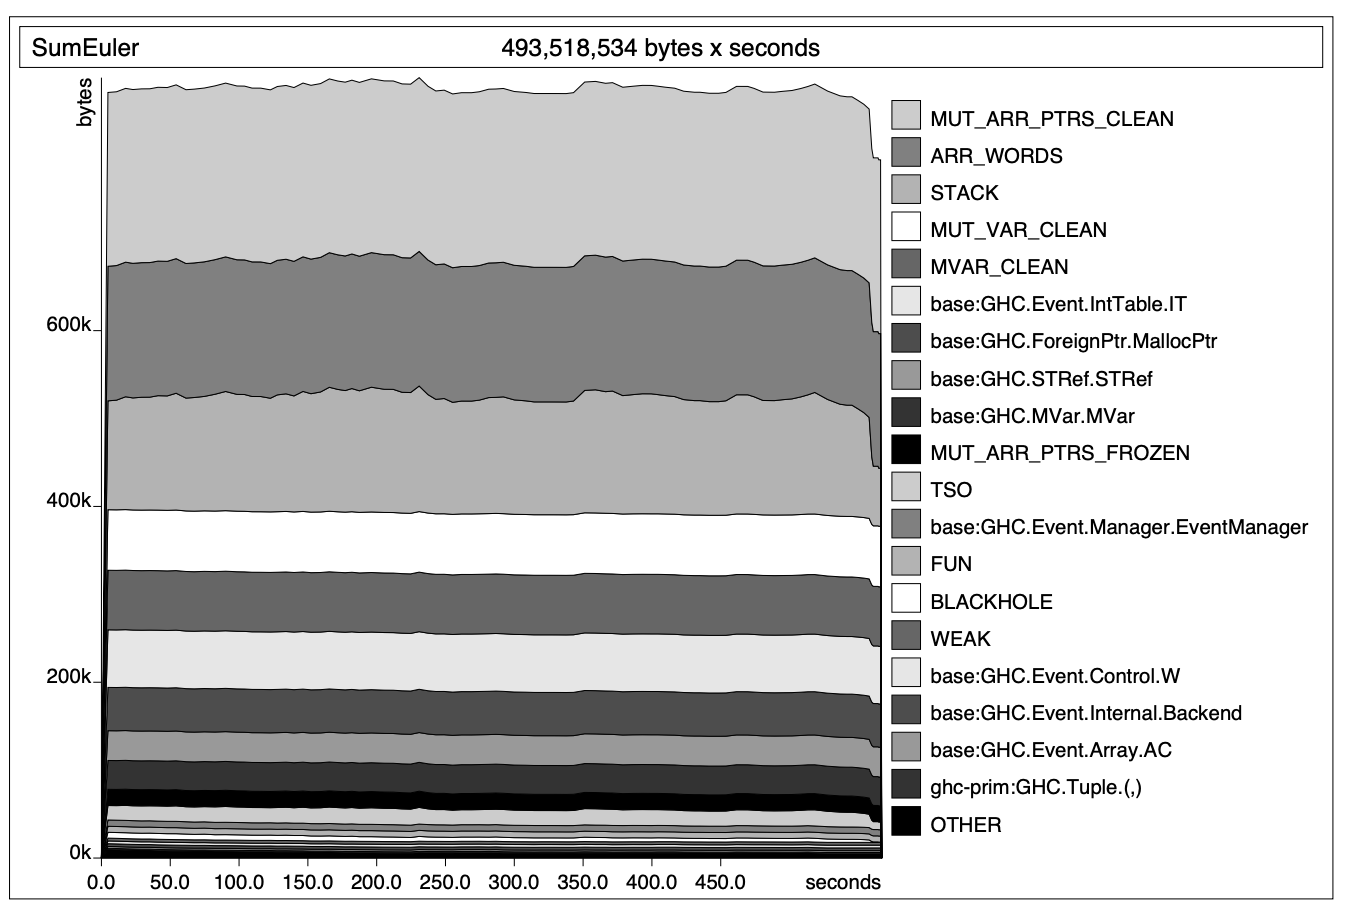
\includegraphics[width=0.75\linewidth]{Paper/images/sumeuler/divconq_hp.png}
    \caption{The allocation rate throughout execution for the divide \& conquer implementation of \lstinline{sumeuler}. Measured by GHC memory profiler.}
    \label{fig:divconq_hp}
\end{figure}

\begin{figure}[!htb]
    \centering
    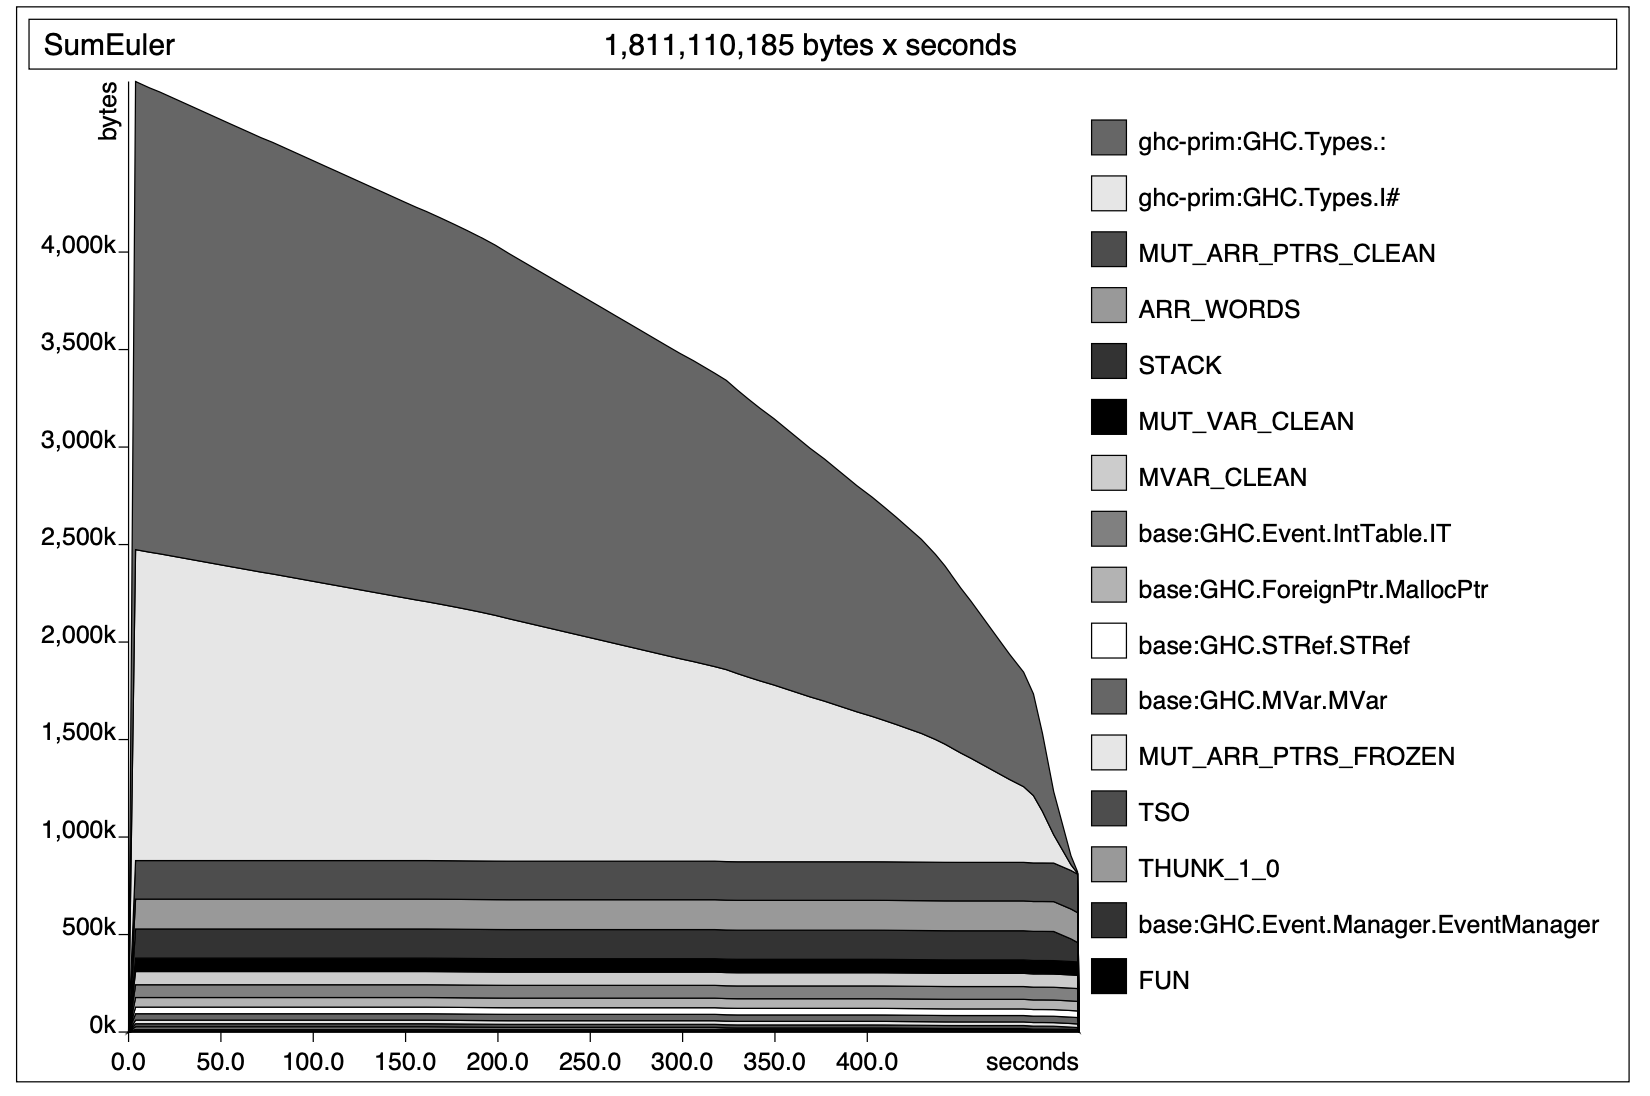
\includegraphics[width=0.75\linewidth]{Paper/images/sumeuler/dp_hp.png}
    \caption{The allocation rate throughout execution for the data parallel implementation of \lstinline{sumeuler}. Measured by GHC memory profiler.}
    \label{fig:dp_hp}
\end{figure}

\begin{figure}[!htb]
    \centering
    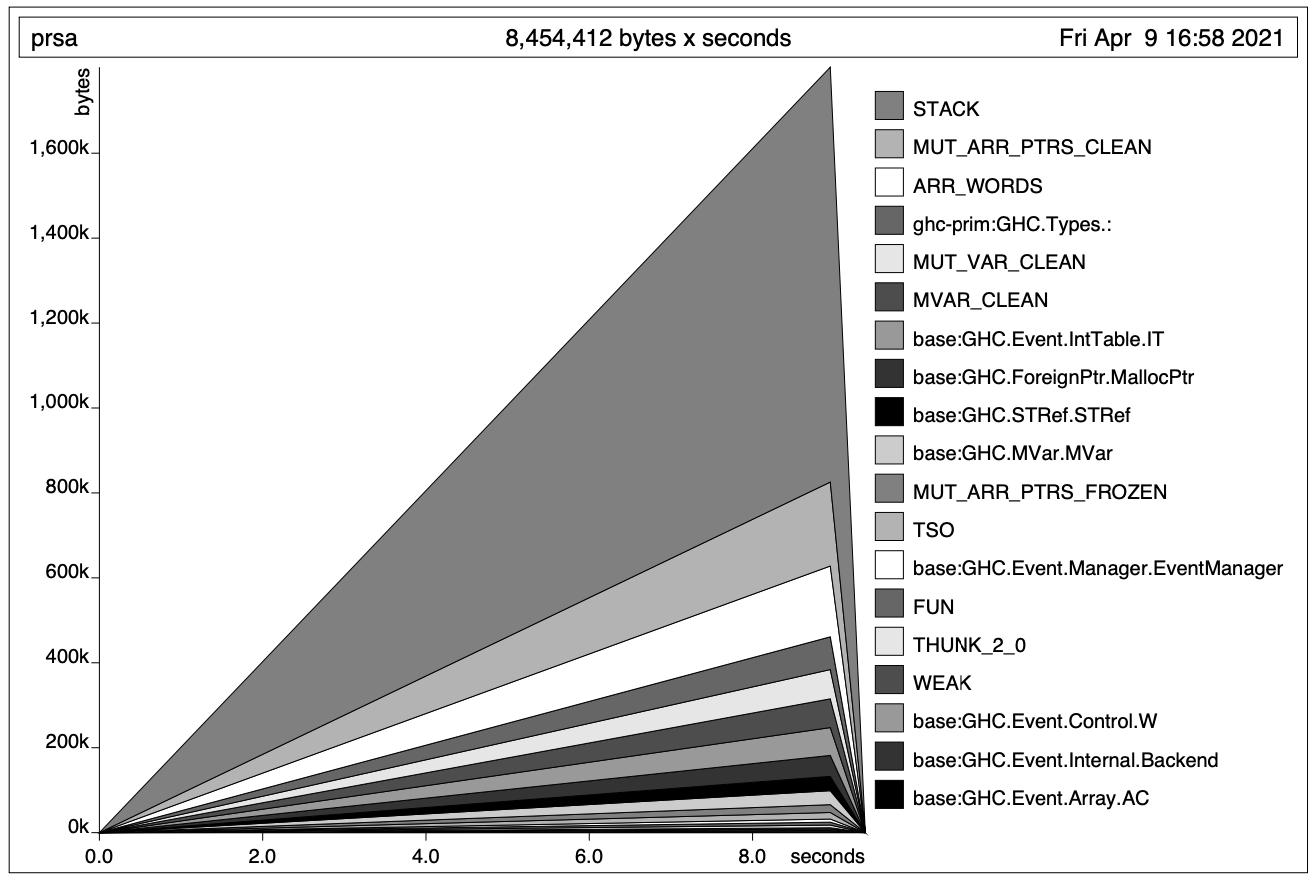
\includegraphics[width=0.75\linewidth]{Paper/images/prsa/prsa_hp.png}
    \caption{The allocation rate throughout execution for \lstinline{prsa}. Measured by GHC memory profiler.}
    \label{fig:prsa_hp}
\end{figure}

Measuring the allocation rates gives possible explanations as to why a shorter runtime was reached, e.g. fewer allocations may lead to faster execution. However, this tool does not feature any NUMA specific metrics that would allow one to realise why the allocation strategy for data parallel appears to be better than DNC. Thus, providing motivation to look deeper into the types of accesses being made, e.g. local \& remote accesses and the source of those accesses, e.g. a thread in region 0 accessing data in region 1. Along with memory accesses, the source of allocations is crucial, and, following on from allocations is the de-allocation of objects. Thus, creating the need to profile the garbage collector that makes it aware of NUMA regions, and specifically, detect the locality of the objects GC threads are processing.

\subsubsection{OS Thread Access Locality}
\label{sec:thread_access_locality}

%Detecting whether a software implementation is effectively exploiting a NUMA architecture creates the need for profiling not only the location of the memory allocated, but also the region the thread resides in. We measure the OS thread access locality via the \textit{numaprof} tool and present access matrices, where an entry $(i, j)$ is the accumulated number of access from \textit{pinned OS threads} residing in region $i$ to region a $j$, e.g. $(i, i)$ is a local access, remote otherwise. All profiles are available at \textbf{UPLOAD LINK TO SOMEWHERE} and includes the numerical data to produce the matrices.

\Cref{fig:access_divConq} shows the heat-map for the DNC implementation of \lstinline{sumeuler}. Across the diagonal there is a good indication of local access being made, indicated by the more apparent shade of purple as opposed to the blue regions. This only equates to 28.7\% of the access by pinned OS threads being made local. Observing the strong colour of red along column 7 indicates many accesses are being made. With 82\% of all memory accesses are to this region. This introduces some questions as to why this occurs, are there many allocations made within this region? is this a shared data structure? Some insight into this already could be answered by the existing region locality implementation in GHC. Allocations are often done in order to maximise locality. Thus, the purple strip may correspond to per region worker local data, e.g. intermediate lists produced.

\Cref{fig:access_dp} shows the heat-map for the data parallel implementation of \lstinline{sumeuler}. Similar to \Cref{fig:access_dp}, there is a good indication of local accesses being made. However, there we observe a 0.9\% increase in local access by pinned OS threads, resulting in 29.6\%, being made which could provide further insight into why the runtime was slightly improved upon. The same issue appears with the red strip however, albeit in region 2. Also showing that 81\% of \textbf{all} memory accesses being made to this region. Thus, the same questions arise and hence provided motivation to extend \textit{numaprof} to incorporate the \textit{allocation locality}. Since the strip is common amongst both profiles, this could perhaps be due to this is where the initial tasks are sparked and hence many accesses may be made to the region, either because (A) some data residing in a task is allocated (B) lots of steal requests to this region. However, since \textit{numaprof} resides at \textbf{OS} level of the stack, and thus, one cannot precisely determine exactly the cause of the remote accesses, because this information resides at the language implementation level, e.g. the OS has no concept of what a Haskell spark is.

\Cref{fig:prsa_access} shows the heat-map for \lstinline{prsa}. Results show that a very small amount of accesses are made by pinned OS threads are local, e.g. 22.9\%. Again, there is a common red strip on the profile, equating to 89.4\% of \textbf{all} memory accesses, thus implicating that many allocations have been made in this area. The \lstinline{prsa} benchmark is compute intensive by nature and thus one does not expect GHC worker threads to be the source of most of the allocations. This illuminates a key challenge for compute intensive benchmarks. As this type of benchmark often features such few allocations, thus creating the need to ensure data that is allocated is appropriately copied and distributed amongst regions, if appropriate, so GHC worker threads do not have to be the source of many remote accesses as the data could be moved closer to the thread. However, detecting this itself within the runtime system would be very challenging, and, specifically, knowing when the remote accesses are becoming an issue.

\begin{figure*}[!htb]
    \centering
    \begin{multicols}{3}
    \caption{DNC \lstinline{sumeuler} access heat-map. Measured by \textit{numaprof}.}
    \label{fig:access_divConq}
    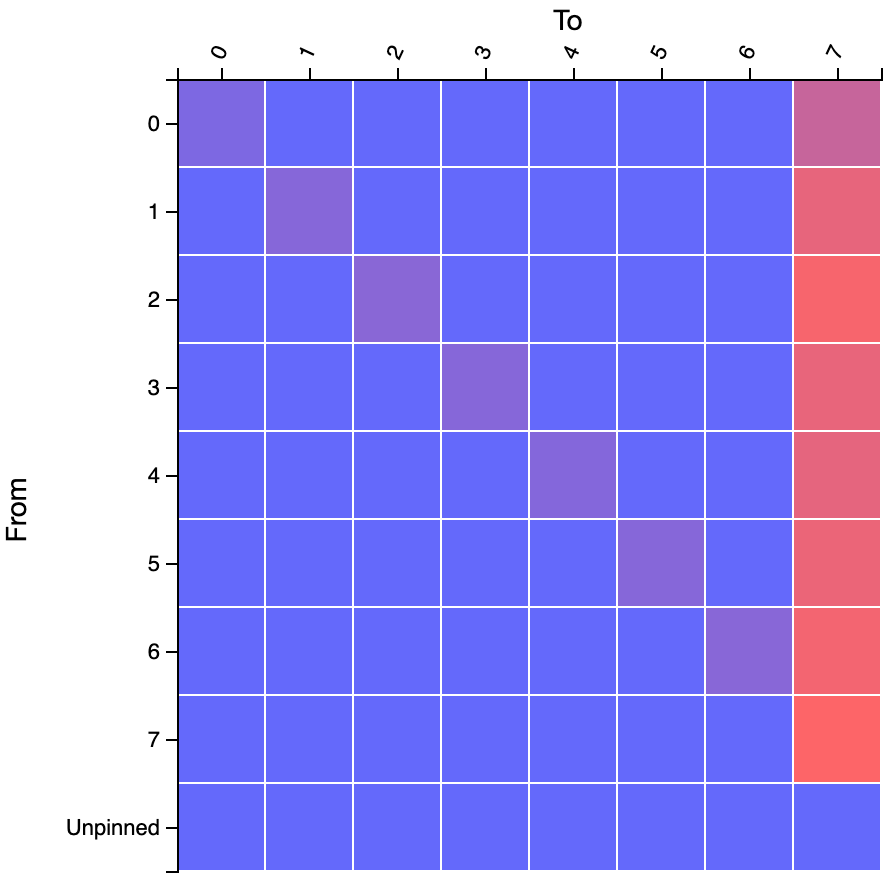
\includegraphics[width=\linewidth]{Paper/images/sumeuler/divconq_access.png}\par
    \caption{Data parallel \lstinline{sumeuler} access heat-map. Measured by \textit{numaprof}.}
    \label{fig:access_dp}
    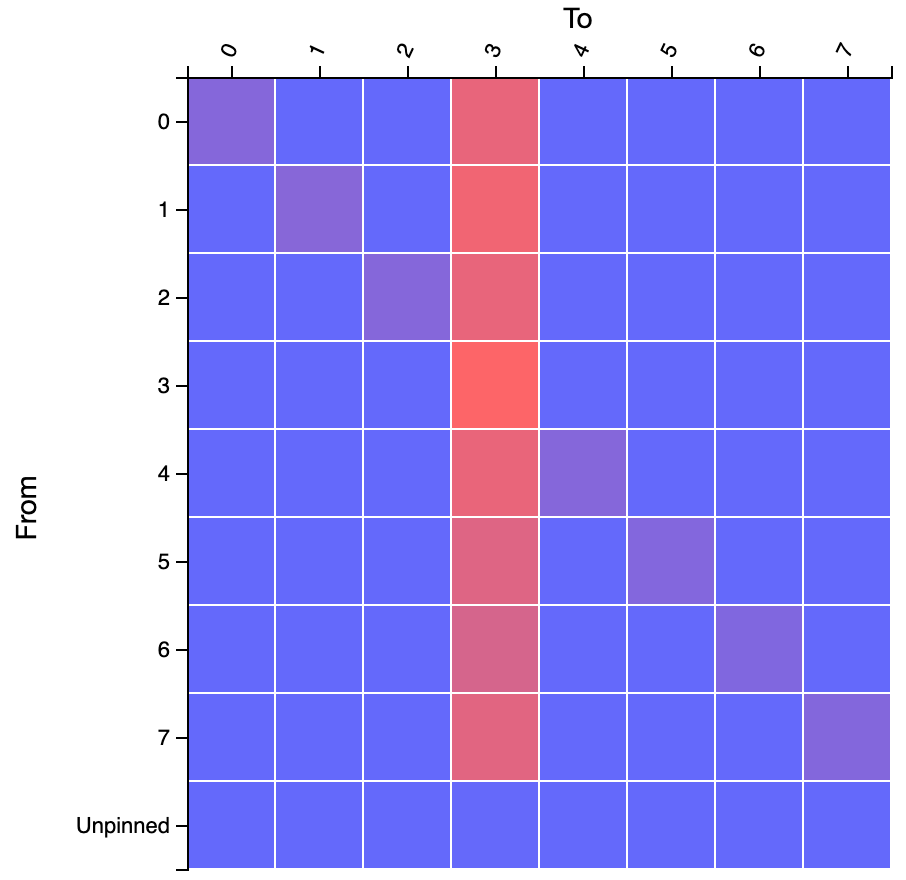
\includegraphics[width=\linewidth]{Paper/images/sumeuler/dp_access.png}\par
    \caption{\lstinline{prsa} access heat-map. Measured by \textit{numaprof}.}
    \label{fig:prsa_access}
    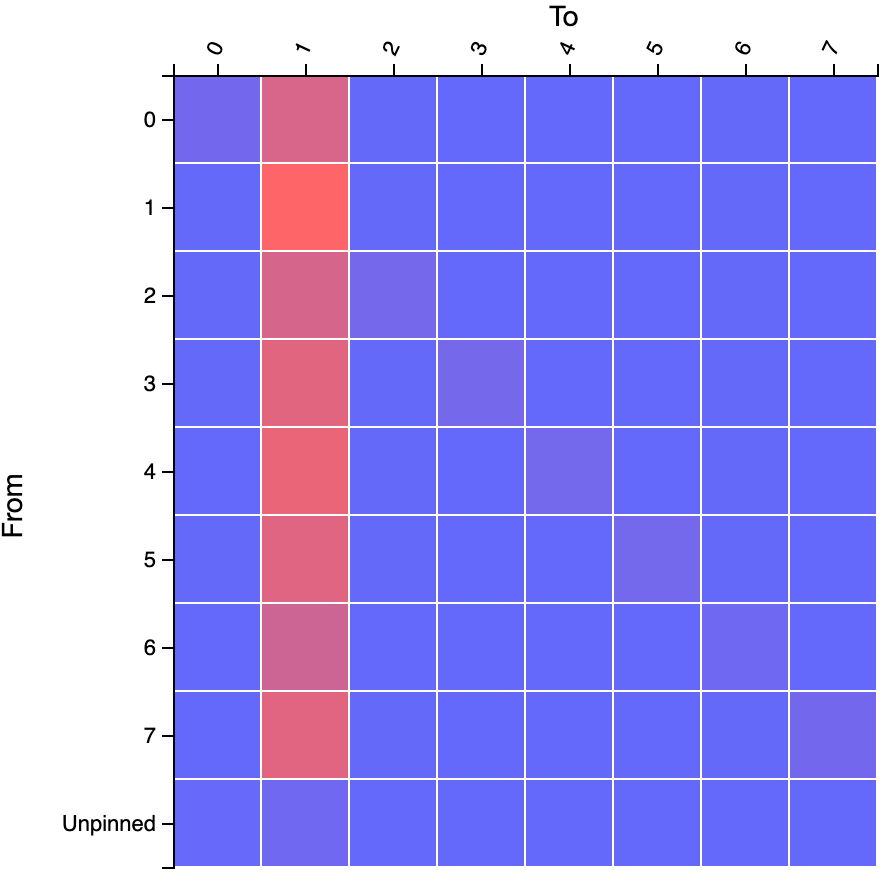
\includegraphics[width=\linewidth]{Paper/images/prsa/prsa_access.png}\par
    \end{multicols}{3}
   % \caption{On the left is static set of objects GC threads process, the middle is generation 1 objects and the right being generation 2 for DNC \lstinline{sumeuler}}
%\label{fig:dnc_static}
\end{figure*}

%\begin{figure}[!htb]
%    \centering
%    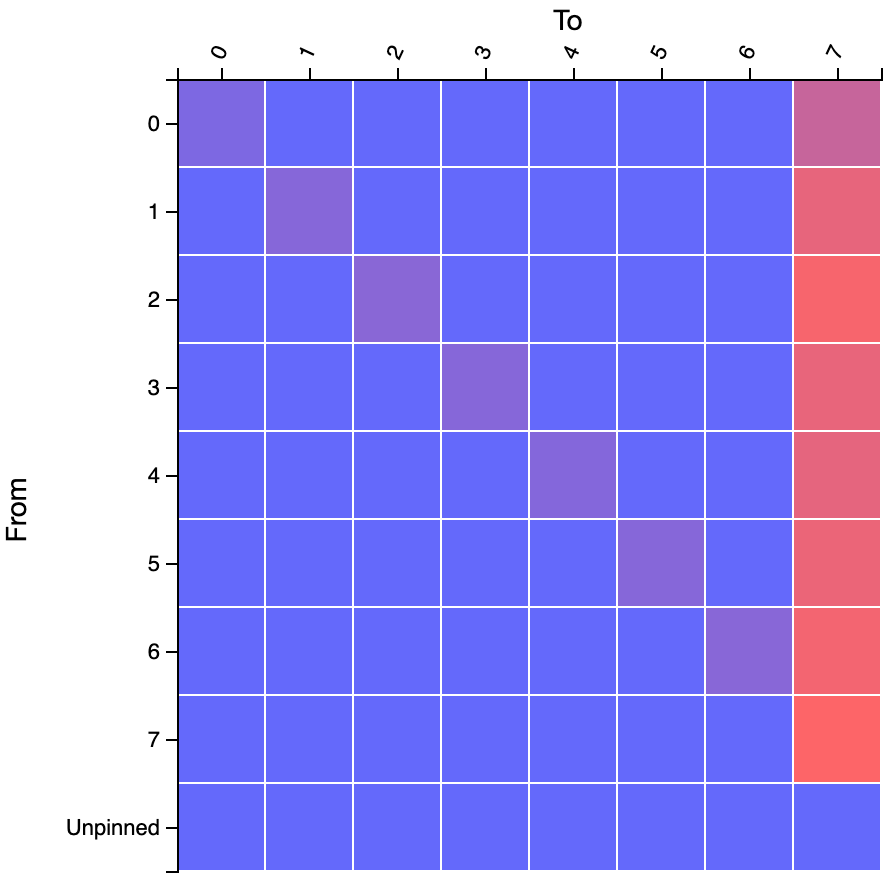
\includegraphics[width=0.6\linewidth]{Paper/images/sumeuler/divconq_access.png}
%    \caption{Access Matrix for Divide \& Conquer \lstinline{sumeuler}. 28.7\% of all accesses made by pinned OS threads are local.}
%    \label{fig:access_divConq}
%\end{figure}

%\begin{figure}[!htb]
%    \centering
%    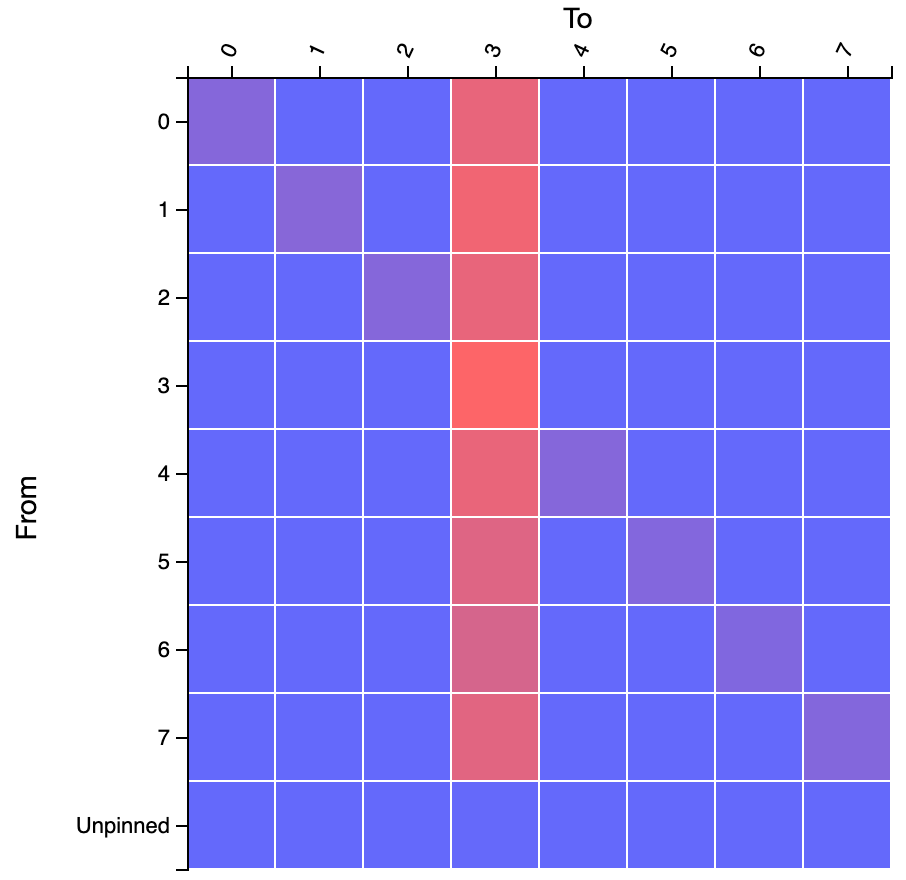
\includegraphics[width=0.6\linewidth]{Paper/images/sumeuler/dp_access.png}
%    \caption{Access matrix for data parallel \lstinline{sumeuler}. 29.6\% of all accesses made %by pinned OS threads are local.}
%    \label{fig:access_dp}
%\end{figure}

%\begin{figure}[!htb]
%    \centering
%%    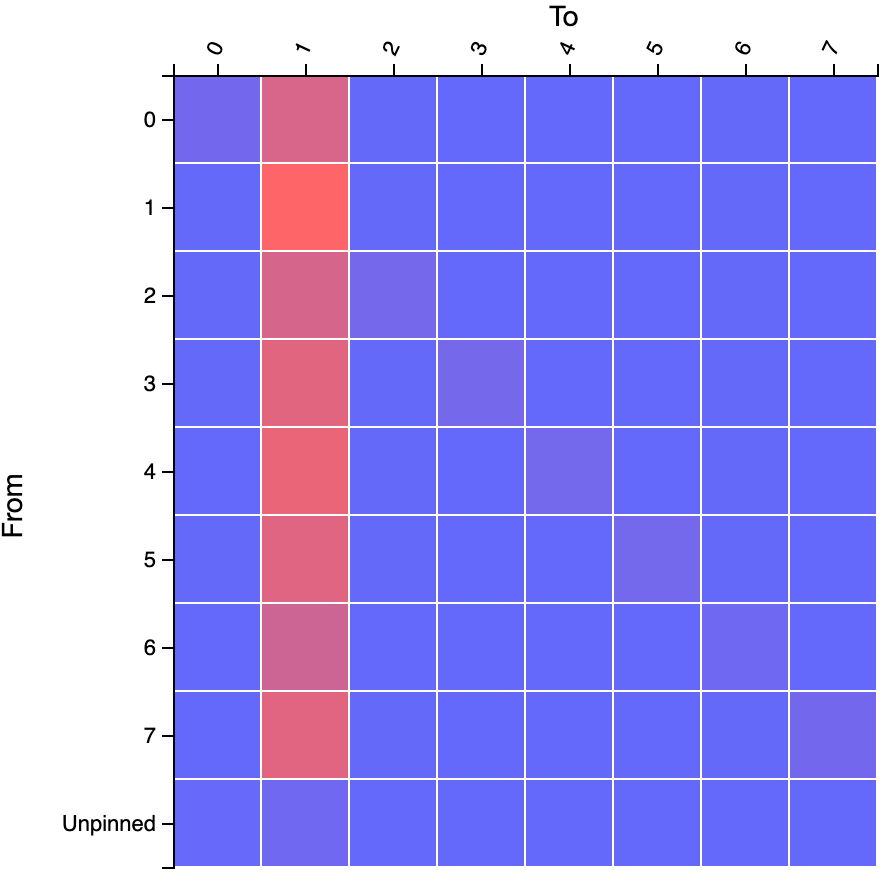
\includegraphics[width=0.6\linewidth]{Paper/images/prsa/prsa_access.png}
%    \caption{Access matrix for \lstinline{prsa}. 22.9\% of all accesses made by pinned OS threads are local.}
%    \label{fig:prsa_access}
%\end{figure}

It is not clear if the high access rates to a particular region, common to each of the figures, e.g. the red strip, are causing any saturation of the memory controllers or the on-chip interconnect. To determine this would require detailed bandwidth measurements which can be obtained from easily from \textit{VTune}. However, the architecture used in the work was AMD and hence could not be achievable. However, if this was to be the case, then this strengthens the case for NUMA architectures, as one is achieving runtime improvements of around (10-20\%) whilst only making 29.6\% of the accesses being made local. Thus, there is still a great deal of work required in GHC to improve upon this locality and hence can provide better performance, given reasonable access patterns and load balance.

\subsubsection{NUMA Distance Accesses}
\label{sec:numa_distance_accesses}

%Arising from a NUMA architecture comes varying processor latency's for reading/writing to memory. Local regions grant the fastest access, with the exception being when load imbalance issues arise, and remote regions are slower to access and streamed to at lower bandwidth. However, not \textbf{all} accesses to particular regions cost the same amount in terms of latency, e.g \Cref{fig:distance} shows the latency's for Togian. This implicates a need to ensure that allocations should always at least attempt to allocate in the region which is closest to its own in terms of latency's and opting for the highest latency's should only be done when load imbalance issues on any surrounding regions which have shorter access latency's. This metric is measured by \textit{numaprof}.

\Cref{fig:sumeuler_dist} shows the NUMA distance access counts for both DNC \& data parallel \lstinline{sumeuler}. For DNC, 28.7\% of all the memory accesses are done within the same region, indicated by the bar-chart with label 10. It turns out that most of the accesses made are at a distance of 16, equating to 41.6\%, thus making some sound access patterns. Finally, the distance factor of 22 having the second highest access rates, with around 29.7\%. Thus possibly contributing to DNC's poorer runtime compared to data parallel. For data parallel, 29.6\% of the accesses are local, e.g. distance factor of 10. Similar to DNC, most of the accesses are done at a distance factor of 16, with around 41.3\% of all accesses being at said distance. Finally, the distance factor of 22 shows the lowest percentage of accesses, 29.1\% of all memory accesses. Although only a 0.7\% increase from the local accesses from a distance factor of 22, given that accessing local memory can be read/written to much faster, e.g. 1.6 to 2.2 times, thus, possibly again, possibly explaining the improved runtime foe the data parallel implementation.

\Cref{fig:prsa_dist} shows the NUMA distance access counts for \lstinline{prsa}. Local accesess appear to be the least common, equating to 23.9\% of all accesses. The most common type of access is at a distance of 16, with 45.3\% of the total accesses. Finally, the distance factor of 22 having 30.8\%. A possible explanation for this low amount of local accesses, could be down to such few allocations are made by GHC worker threads, as the benchmark is compute intensive, thus leading to most of the data allocated in the initial tasks sparked, and could be the source of many remote accesses.

\begin{figure}[!htb]
    \centering
    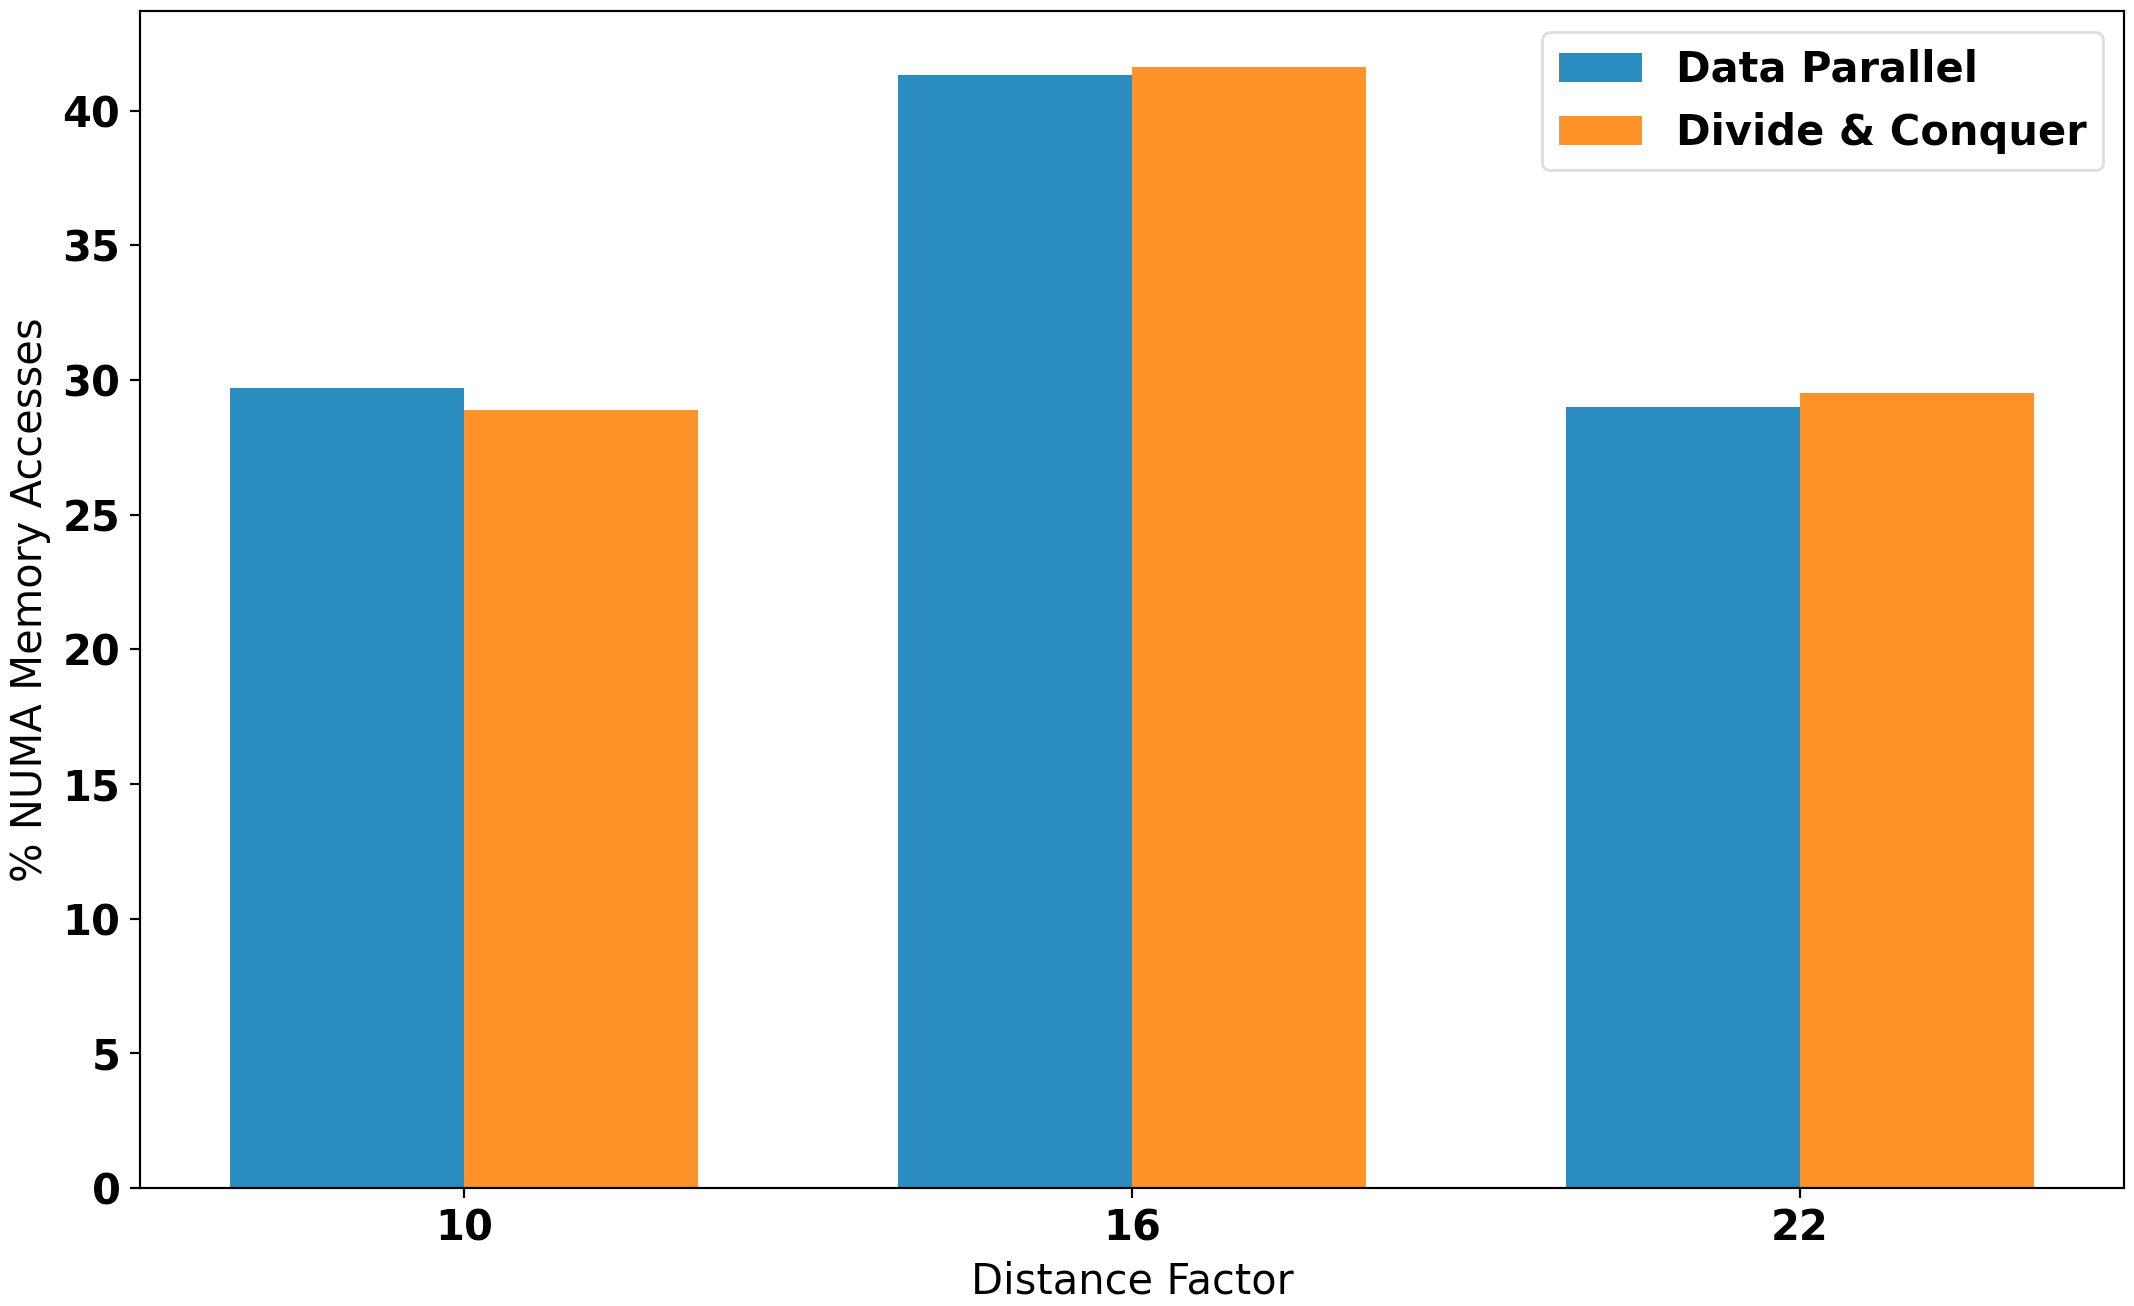
\includegraphics[width=\linewidth]{Paper/images/sumeuler/sumeuler_dist.png}
    \caption{OS thread NUMA distance counts from the \lstinline{sumeuler} benchmark. Measured by \textit{numaprof}.}
    \label{fig:sumeuler_dist}
\end{figure}

\begin{figure}[!htb]
    \centering
    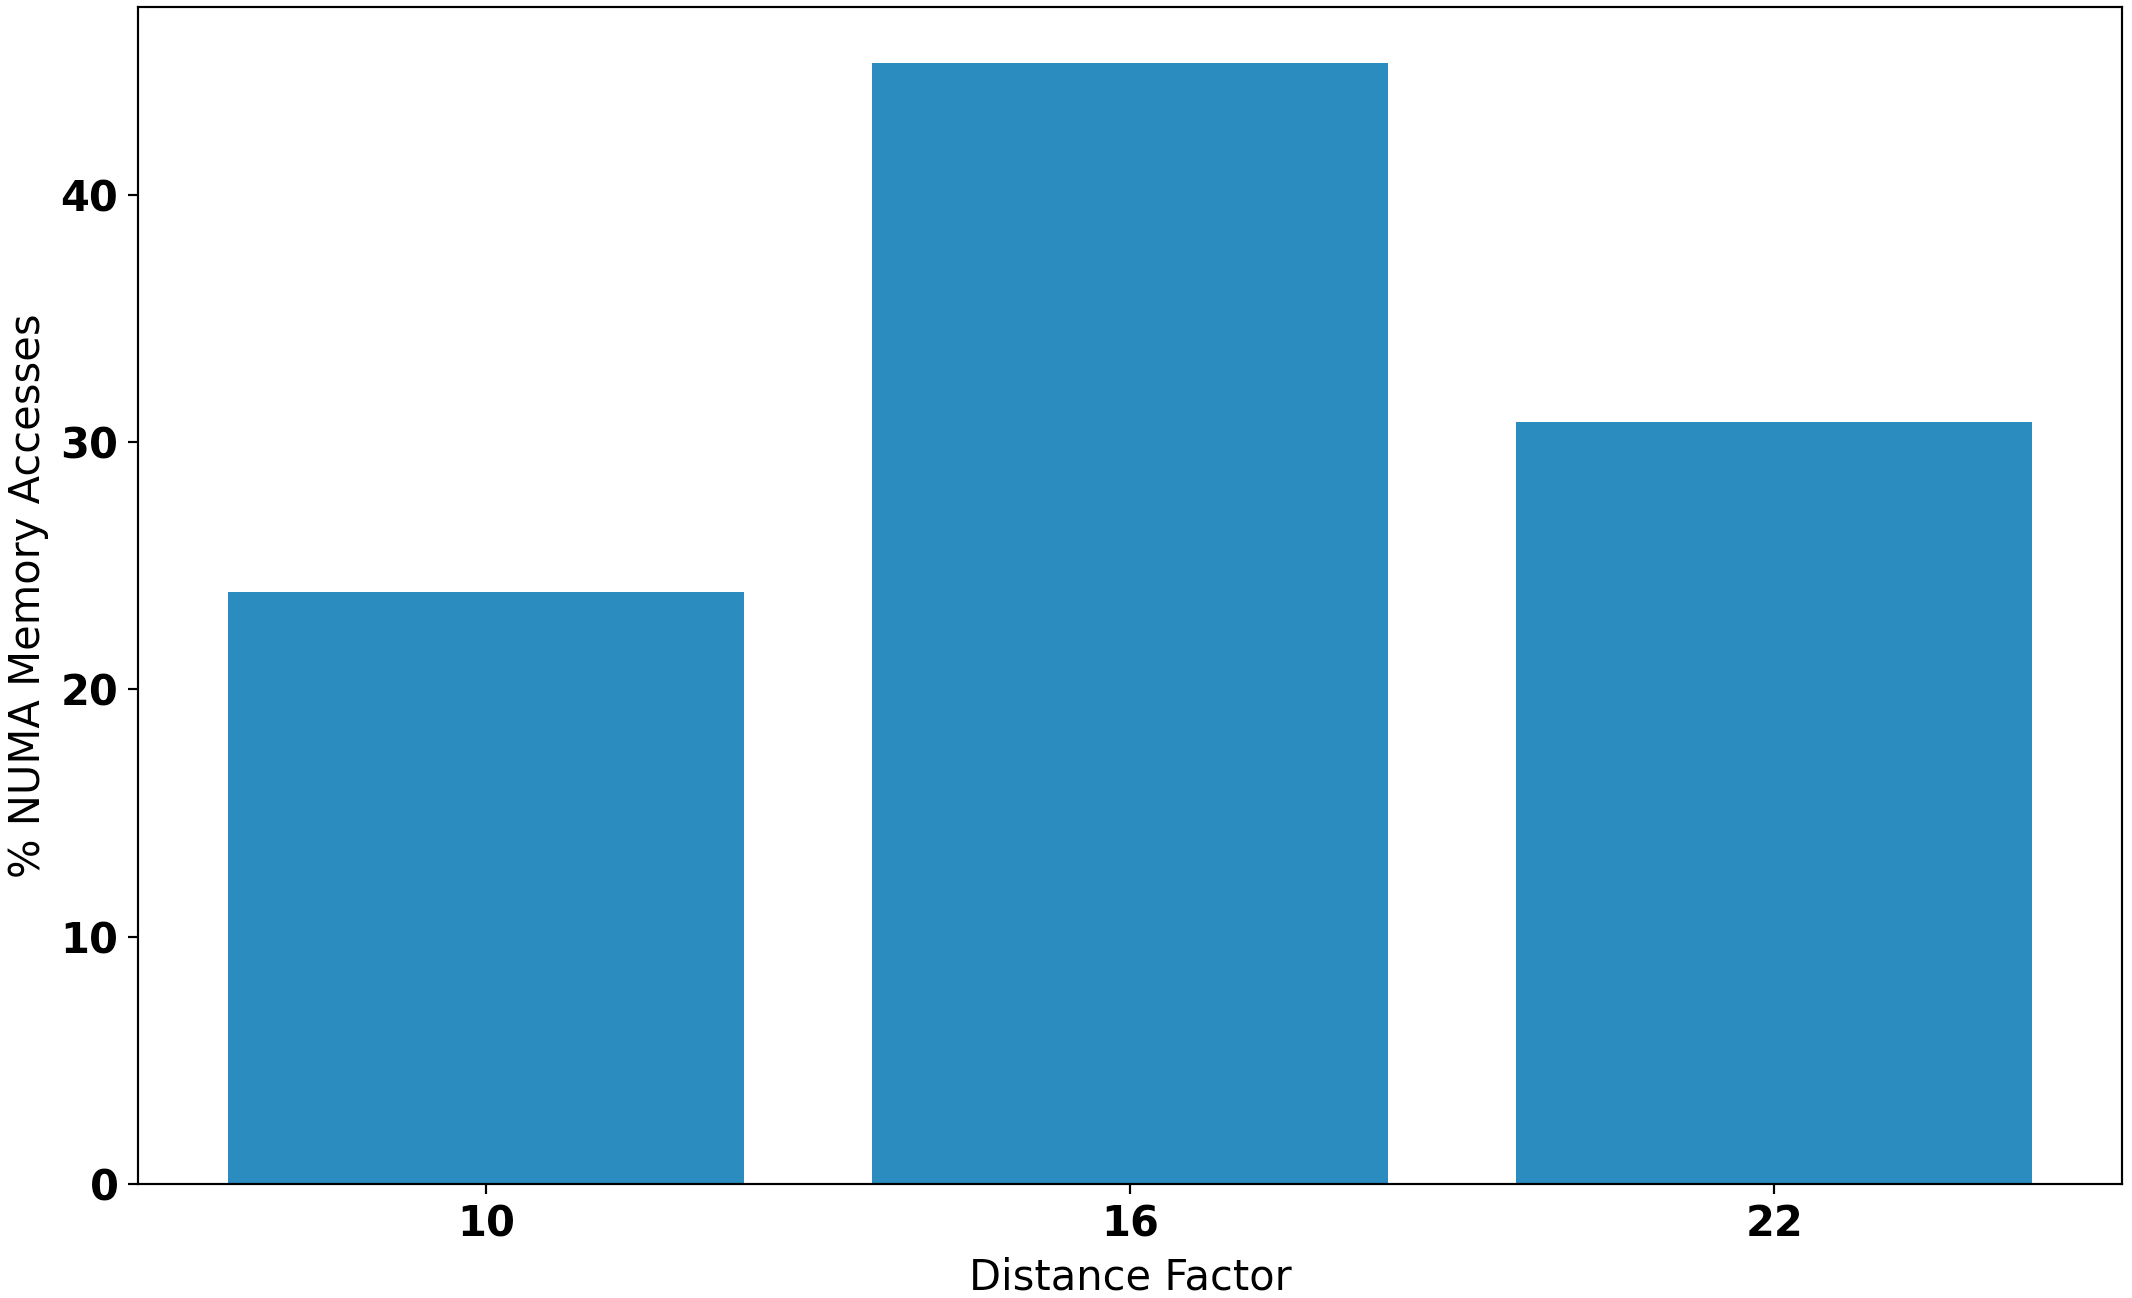
\includegraphics[width=\linewidth]{Paper/images/prsa/prsa_dist.png}
    \caption{OS thread NUMA distance counts from the \lstinline{prsa} benchmark. Measured by \textit{numaprof}.}
    \label{fig:prsa_dist}
\end{figure}

\subsection{Summary}
\label{sec:summary}

The metrics primarily focused on allocation from existing tools present useful knowledge with how to GHC behaves over a NUMA. Across the 3 benchmarks used, there appears to be a common case of a lot of accesses to a region, indicated by the strong colour of red.

However, this did raise some questions. The access matrix only gives information about whether access is local and where it comes from. This on its own can be a fairly good indicator of the allocations occuring in the application, e.g. lots of accesses to a particular region implies high allocations. But, precise details is necessary with regards to the allocations as it is a crucial factor when writing applications that execute over NUMA.

\section{Profiling Allocation \\ Locality in numaprof}
\label{sec:extnumaprof}

This section outlines the extension to numaprof to record allocation locality, and illustrates the profiles produced.

A sufficient tool that was able to encapsulate the allocation locality per region was not discovered. There are two possible sources to implement this profiling information: the GHC runtime itself and \textit{numaprof}. \textit{numaprof} was chosen as it already featured a \lstinline{malloc} tracker from a previous tool - MALT\cite{DBLP:conf/oopsla/ValatCJ17}, implemented by the same authors. MALT tracks the location where the data was allocated. Thus, the only extensions that were required were to track the location of the calling thread and to (1) store this in an access matrix at runtime (2) integrate it into the \textit{numaprof} web based UI. The specific implementation is freely available on github\footnote{https://github.com/ruairidhm98/numaprof} in branch "AllocationLocality". GHC would have been a good choice, perhaps better, however, making extensions to the GHC RTS is far from trivial and is difficult to know if the extensions would actually be correct.

\Cref{fig:dp_alloc} shows the allocation heat-map for data parallel \lstinline{sumeuler}. All allocations are done locally by GHC worker threads and correspond with the region locality features implemented within GHC, e.g. locality allocation optimisations. However, although not clear in the picture as the specific numerical data is not present, but, of all unpinned allocations done e.g. the bottom row in the matrix, entry $(3, 8)$ amounts to 5040153 bytes allocated, corresponding to 97\% of the unpinned allocations. Thus, the main thread will perhaps be causing these initial allocations via sparking tasks and the source of many remote accesses are from GHC worker threads which are pinned to regions and require some data from the initial closure allocated by the main thread.

\Cref{fig:dp_alloc} shows the allocation heat-map for data parallel \lstinline{sumeuler}. Similar to DNC, all allocations are done local by GHC worker threads. A similar situation, with 83\% (GET CORRECT NUM) of the unpinned allocations down within region 3. The tool highlights this via the more apparent shade of purple in entry the unpinned entry for region 3. The main thread in GHC is not pinned to a specific region and thus the allocations made by this thread are all along the bottom row. Thus, one could infer that the large amount of bytes allocated within region 3 must be the initial tasks sparked by the main thread. Thus, causing so many accesses in \Cref{fig:access_dp}.

\Cref{fig:prsa_alloc} shows the allocation heat-map for \lstinline{prsa}. Similar to \lstinline{sumeuler}, all allocations done by GHC worker threads are local, illuminated by the colour blue across the diagonal. We expect their to be less allocations by worker threads for \lstinline{prsa} as it is a compute intensive benchmark. Thus, one can suspect that the strong red colour in entry $(1, 8)$ is to do with the main thread sparking tasks for the workers, and, thus leading to the high access rates seen in \Cref{fig:prsa_access}.



%\begin{figure}[!htb]
%    \centering
%    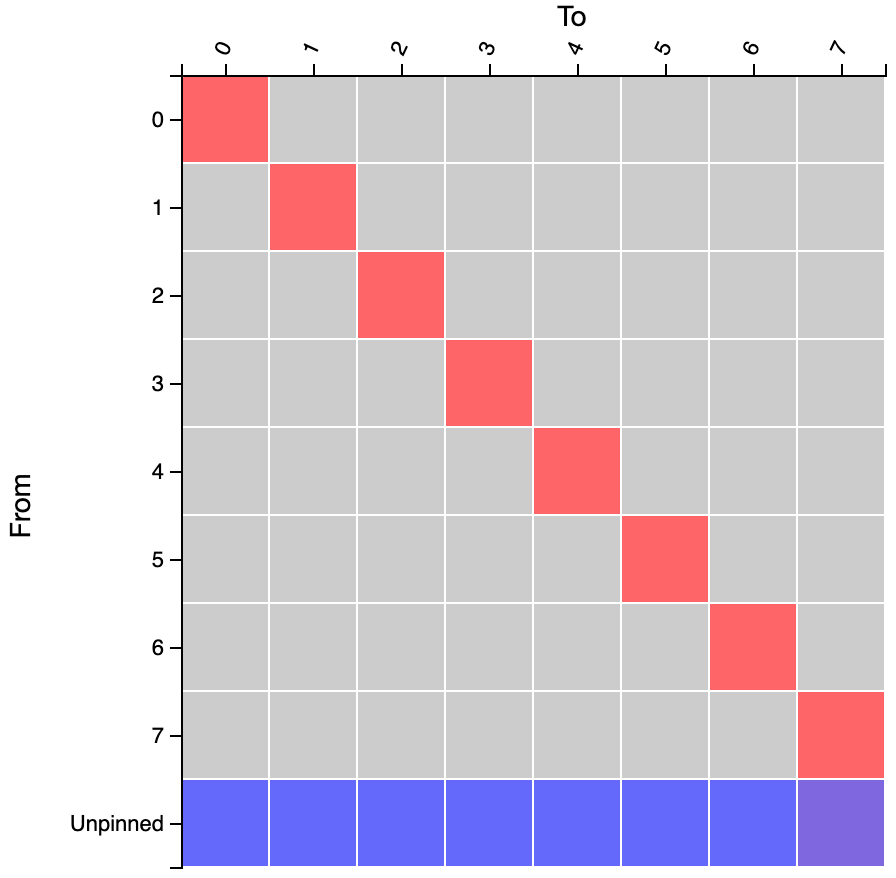
\includegraphics[width=0.6\linewidth]{Paper/images/sumeuler/divconq_alloc.png}
%    \caption{Divide \& Conquer \lstinline{sumeuler} allocation matrix}
%    \label{fig:divconq_alloc}
%\end{figure}

%\begin{figure}[!htb]
%    \centering
%    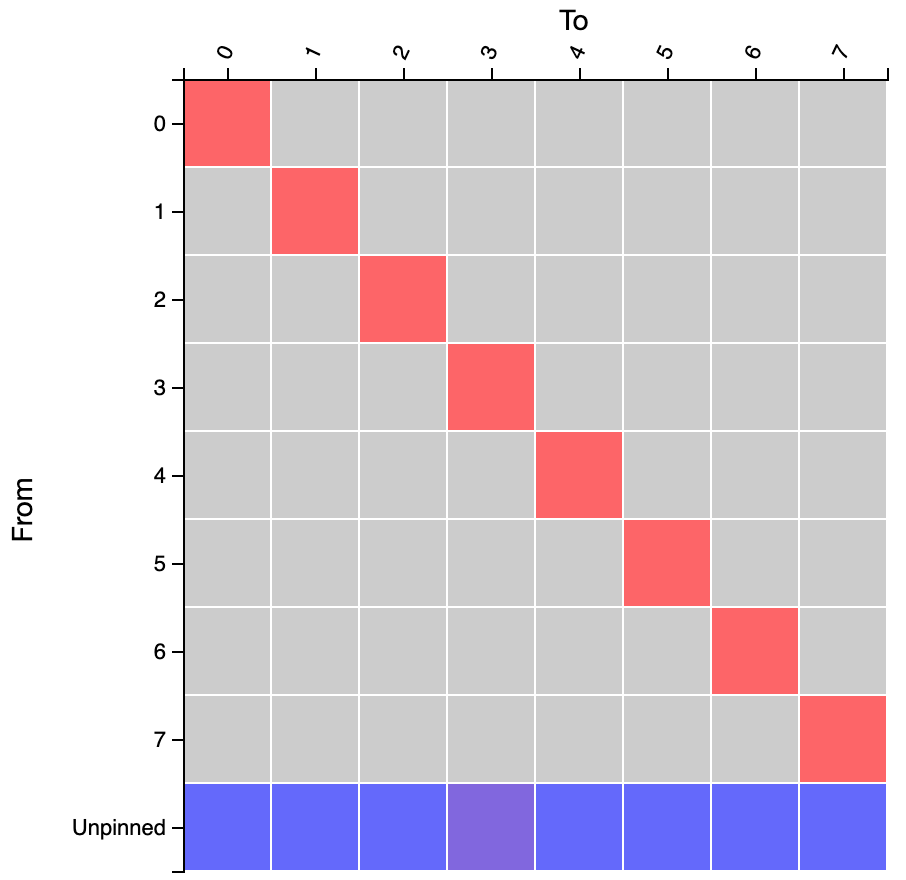
\includegraphics[width=0.6\linewidth]{Paper/images/sumeuler/dp_alloc.png}
%    \caption{Data parallel \lstinline{sumeuler} allocation matrix}
%    \label{fig:dp_alloc}
%\end{figure}

%\begin{figure}[!htb]
%    \centering
%    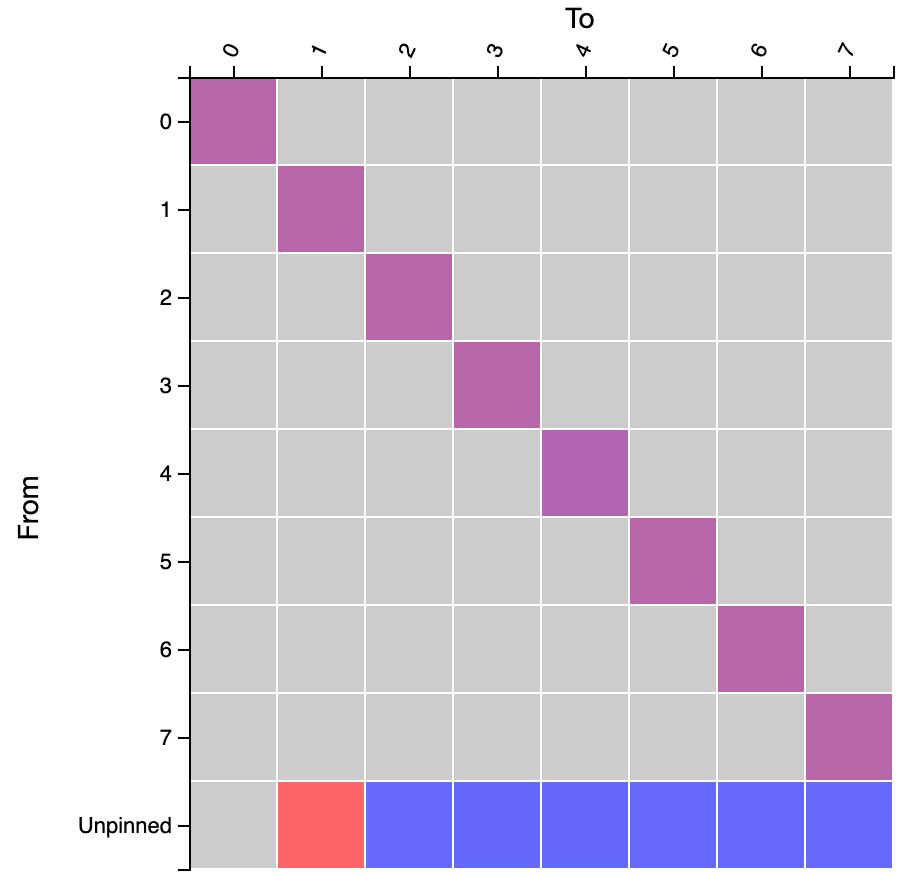
\includegraphics[width=0.6\linewidth]{Paper/images/prsa/prsa_alloc.png}
%    \caption{\lstinline{prsa} allocation matrix}
%    \label{fig:prsa_alloc}
%\end{figure}

These profilers reveal to the runtime system developer the precise locations in the NUMA architecture. Thus, when combined with the \textit{access matrix}, and the OS thread NUMA distance counts are taking into account, indicates if access and allocations are being made in such a manner to minimise latency, e.g. are local, try region at the next distance etc.

However, as the information is collected at the \textbf{OS} level, thus losing any abstractions made within the language implementation and makes it harder to pin point the allocations within the region. It is not certain whether or not the allocations done by GHC worker threads cause load imbalance as all allocations are done locally. \textit{Intel VTune} gives informative details with regards to bandwidth consumption per NUMA region throughout program execution. A sufficient tool that could be used on the AMD server Togian was not discovered and hence limited this work.

The obvious next step is to record this metric in the language runtime system as one can take into account all the abstractions within GHC to profile specific objects and know e.g. which are most costly and those that aren't. The language implementation's runtime system has the most adequately detailed levels of application specific information. Such information in the current implementation turned out to be useful in the sense we can visualise the location of the allocations, but it lacks that next step to reveal what is the underlying issues with specific objects in the runtime system that could perhaps be identified and improved upon.

\section{Profiling NUMA in GHC GC}
\label{sec:extghc}

The GHC GC features an informative profiler\footnote{https://downloads.haskell.org/ghc/latest/docs/html/users\\\_guide/runtime\_control.html} which gives specific details with regards to: bytes moved/copied, frequency, runtimes - overall \& each cycle, closure breakdown etc. However, no NUMA specific statistics have been implemented in time of writing. Thus, extensions were required to do so. We record the \textit{GC frequency} per region and per generation, and, \textit{GC thread locality}. The \textit{GC frequency} encapsulates information with regards to the specific regions where GC is occuring most frequently. Such information is useful as the regions which GC occurs most frequently tends to be regions in which allocations tends to be higher, e.g. there is more work for the GC to do at those regions. This is useful for detecting highly populated regions and hence load imbalance issues that may arise. The latter metric \textit{GC thread locality} is similar to the \textit{access locality} discussed in \Cref{sec:os_tools} as it gives an insight into the locality of the objects each GC thread is processing. The implementation can be found on github\footnote{https://github.com/ruairidhm98/ghc}.

\begin{figure*}[!htb]
    \centering
    \begin{multicols}{3}
    \caption{DNC \lstinline{sumeuler} allocation locality heat-map. Measured by extensions to \textit{numaprof}.}
    \label{fig:divconq_alloc}
    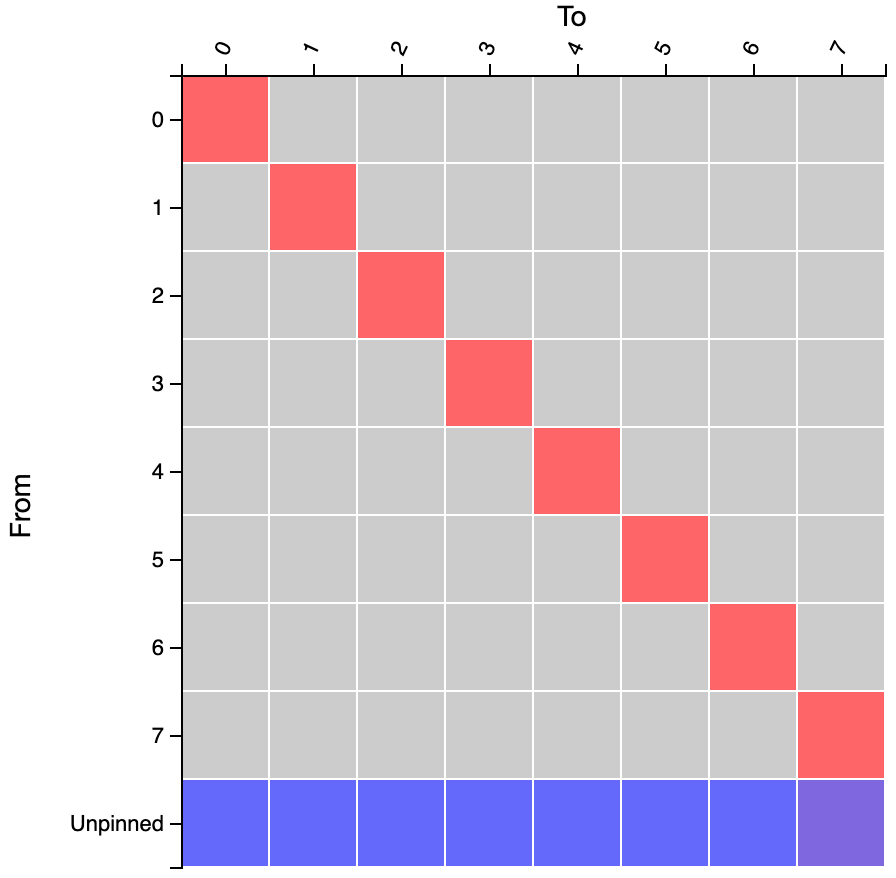
\includegraphics[width=\linewidth]{Paper/images/sumeuler/divconq_alloc.png}\par
    \caption{Data parallel \lstinline{sumeuler} allocation locality heat-map. Measured by extensions to \textit{numaprof}.}
    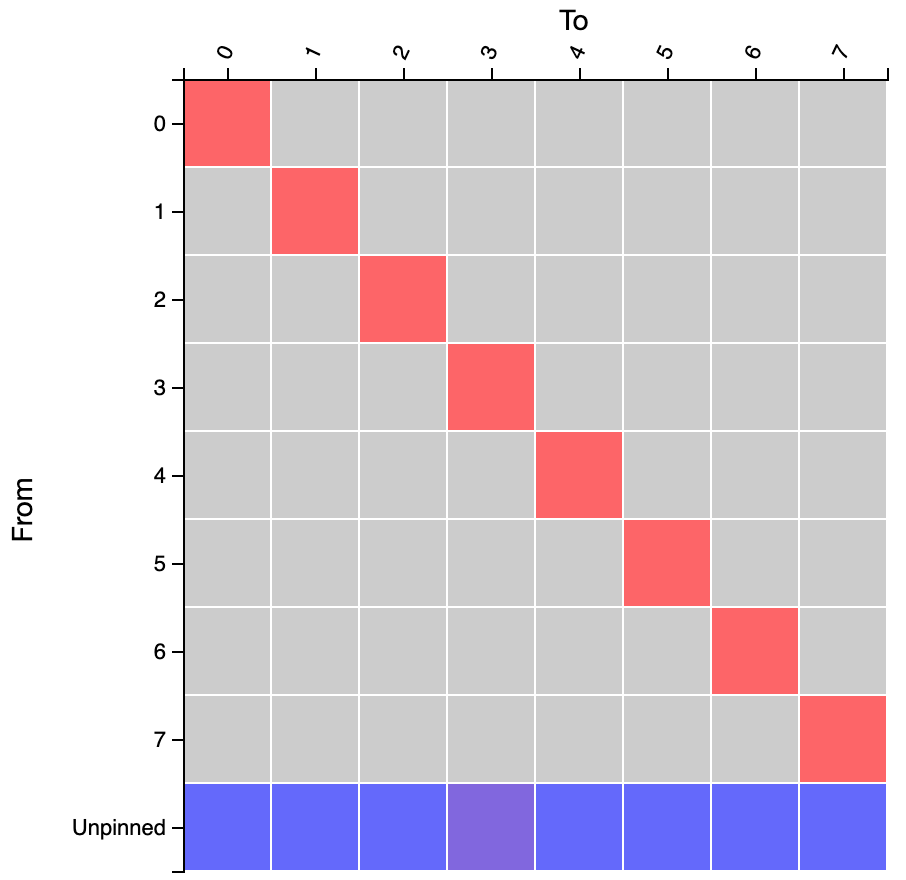
\includegraphics[width=\linewidth]{Paper/images/sumeuler/dp_alloc.png}\par
    \caption{\lstinline{prsa} allocation locality heat-map. Measured by extensions to \textit{numaprof}.}
    \label{fig:prsa_alloc}
    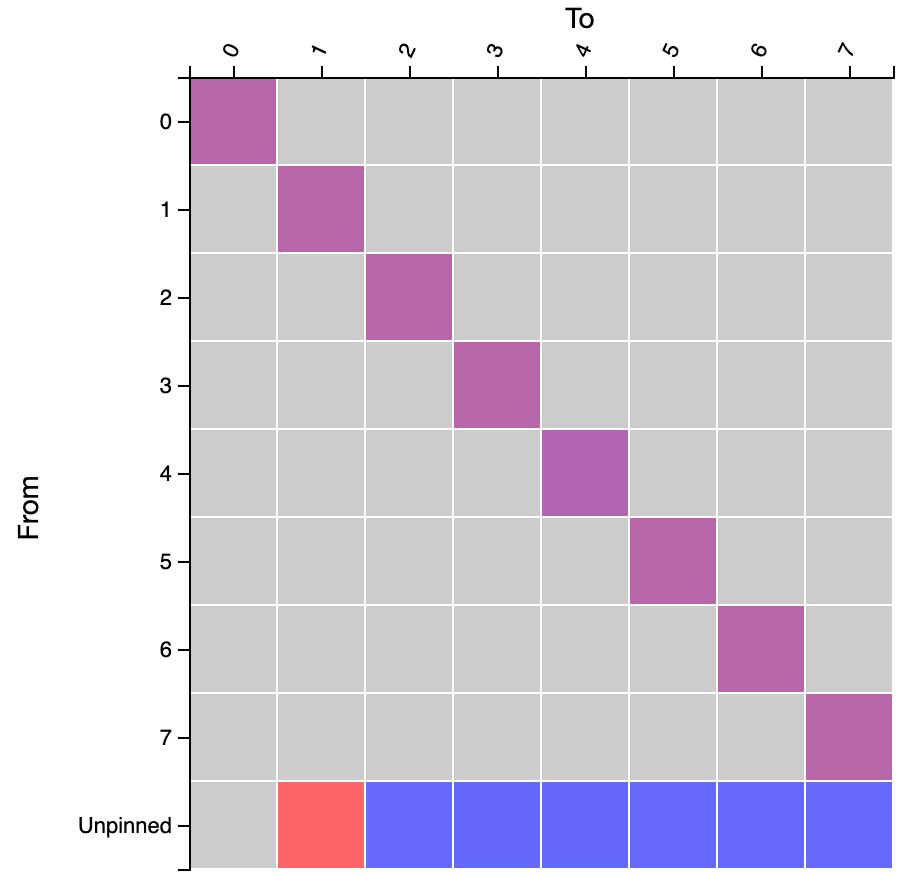
\includegraphics[width=\linewidth]{Paper/images/prsa/prsa_alloc.png}\par
    \end{multicols}{3}
    %\caption{On the left is static set of objects GC threads process, the middle is generation 1 objects and the right being generation 2 for DNC \lstinline{sumeuler}}
    \label{fig:dnc_static}
\end{figure*}

\subsection{Per Region GC Frequency}
\label{sec:frequency}

To implement the \textit{GC frequency}, the information is stored within each Haskell Execution Context (HEC). The GHC GC carries out GC in a manner similar to stop-the-world, however, it generally often only carries out GC in a single HEC, leaving others in normal execution unless explicitly required to carry out a GC. Upon instantiating a new GC cycle, a counter is incremented within the HEC, depending upon which generation its occuring in. Leaving the information to be stored in a HEC is highly advantageous as it incorporates no shared state amongst GC threads, as there is only one GC thread per HEC.

\Cref{table:dnc_freq} shows the garbage collector frequencies per region for the DNC implementation of \lstinline{sumeuler}. A total number of 3983 cycles are carried out in generation 1 and 18 in generation 2. Only a very small amount of major garbage collections take place, e.g. garbage collecting region 2, as well as 1, indicated by only a maximum collections of 4 carried out in region 0. Meanwhile, the minimum number of minor collections being 408. Thus, implicating that perhaps lots of the data allocated by GHC worker threads is short lived data. As illustrated in \Cref{fig:dnc_hp} shows that allocations and allocation rate are fairly constant throughout, thus implicating that a lot of data is temporary and short lived, as e.g., the program wouldn't need to keep allocating otherwise.

\Cref{table:dp_freq} shows the garbage collector frequencies per region for the data parallel implementation of \lstinline{sumeuler}. A total number of 2634 cycles are carried out in generation 1 and 49 in generation 2 Very few major garbage collections take place, with the maximum occuring in region 1, with 11 cycles. Reasons for the increased number of  major cycles could be because most allocations are done earlier within the program as shown in \Cref{fig:dp_hp}, thus leading to objects with long lifetimes. Also, since the total number of cycles for the data parallel implementation is far fewer than DNC, the overhead imposed by the garbage collector is smaller.

\Cref{table:prsa_freq} shows the garbage collector frequencies per region for \lstinline{prsa}. A total number of 647 cycles are carried out in generation 1 and 190 in generation 2. Such few generation 1 cycles could be explained by the nature of the benchmark, e.g. its compute intensive. Therefore, the application doesn't allocate as much memory as \lstinline{sumeuler}. However, generation 2 has far more cycles, even when compared to \Cref{table:dnc_freq} \& \Cref{table:dp_freq}. Thus, implicating many data is long lived in the benchmark.

\begin{table}[!htb]
  \centering
  \resizebox{\linewidth}{!}{
  \footnotesize
  \begin{tabular}{@{}c|cccccccc@{}}

  \makecell{Generation} & \makecell{Region 0} & \makecell{Region 1} & \makecell{Region 2}   & \makecell{Region 3} & \makecell{Region 4} & \makecell{Region 5}   & \makecell{Region 6} & \makecell{Region 7} \\
  \midrule
  1 & 493 & 643 & 461 & 509 & 499 & 408 & 509 & 461 \\
  2 & 4   & 1   & 2   & 3   & 2   & 1   & 2   & 3   \\
  \midrule
  \end{tabular}
  }
  \caption{Garbage Collection frequencies per region for the DNC implementation of \lstinline{sumeuler}. Measured by extensions to GHC GC.}
  \label{table:dnc_freq}
\end{table}

\begin{table}[!htb]
  \centering
  \resizebox{\linewidth}{!}{
  \footnotesize
  \begin{tabular}{@{}c|cccccccc@{}}
  \makecell{Generation} & \makecell{Region 0} & \makecell{Region 1} & \makecell{Region 2} & \makecell{Region 3} & \makecell{Region 4} & \makecell{Region 5} & \makecell{Region 6} & \makecell{Region 7} \\
  \midrule
    1 & 390 & 165 & 175 & 432 & 345 & 288 & 488 & 351 \\
    2 & 11  & 7   & 6   & 4   & 6   & 6   & 5   & 4   \\
  \midrule
  \end{tabular}
  }
  \caption{Garbage Collection frequencies per region for data parallel implementation of \lstinline{sumeuler}. Measured by extensions to GHC GC.}
  \label{table:dp_freq}
\end{table}

\begin{table}[!htb]
  \centering
  \resizebox{\linewidth}{!}{
  \footnotesize
  \begin{tabular}{@{}c|cccccccc@{}}
  \makecell{Generation} & \makecell{Region 0} & \makecell{Region 1} & \makecell{Region 2} & \makecell{Region 3} & \makecell{Region 4} & \makecell{Region 5} & \makecell{Region 6} & \makecell{Region 7} \\
  \midrule
  1 & 153 & 81 & 80 & 90 & 68 & 70 & 35 & 70 \\
  2 & 49  & 24 & 23 & 22 & 23 & 20 & 10 & 19 \\
  \midrule
  \end{tabular}
  }
  \caption{Garbage Collection frequencies per region for \lstinline{prsa}. Measured by extensions to GHC GC.}
  \label{table:prsa_freq}
\end{table}

Recording the runtimes of each collection would of perhaps improved upon this and producing a violin plot as a result, illuminating the GC cycle runtime distribution. Such information would implicate if GC threads are processing lots of remote objects as they would take longer to access. However, to gain an insight into which the locations of the objects garbage collector threads are processing resulted in extending GHC to keep track of this information.

\subsection{GHC GC Thread Locality}
\label{sec:gc_thread_locality}

To implement the \textit{GC thread locality}, the information again, resides within each HEC, for the same reasons, e.g. no synchronisation required as accesses are made by at most one thread. Encapsulating the new profiling information required discovering the location of an object a GC thread is processing as well as the location of the thread itself. Although overhead was reduced by avoiding synchronisation and coordination amongst other threads to encapsulate this information, the implementation still imposes much overhead as it relies on expensive \lstinline{syscalls} to discover the location of the data. The location of the thread is already known before hand as it is pinned to the region in which the HEC it belongs to resides. Making the profiler efficient was not a core aim of this project and hence was avoided for time reasons, however, a simple and efficient extensions would be to cache the value of \lstinline{syscalls}.

\Cref{fig:dnc_static} shows the heat maps corresponding to the locations garbage collector threads are processing objects in the DNC implementation of \lstinline{sumeuler}. \Cref{fig:dncc_static} is for static allocations and evidently, shows no sign of region locality, as the accesses are distributed amongst all regions and there appears to be no strong locality sense. Equating to 15.0\% of static objects being processed locally To some extent this is to be expected as static allocations don't take into account the NUMA regions which GC threads reside in. Although, the allocation placement would be impossible to reason about statically, the ability to detect this information in the runtime is arguably crucial, since the GC could move data closer to threads that need it most, or e.g. copy it and distribute amongst regions if it is a shared object. \Cref{fig:dnc_gen1} is for objects in generation 1 and shows that 86.4\% of the objects are processed locally. \Cref{fig:dp_gen2} is for objects in generation 2 and shows that 93.2\% of all objects are processed locally. Reasons for such high locality rates could be due to the lists are generated once a worker thread has instantiated it, as the implementation is interval based.

\Cref{fig:dp_static} shows the heat maps corresponding to the locations garbage collector threads are processing objects in the data parallel implementation of \lstinline{sumeuler}. \Cref{fig:dpp_static} is for static allocations and shows similar features to \Cref{fig:dnc_static}, e.g. there appears to be multiple regions in which data is distributed and no strong sense of locality. Only, 13.2\% of static objects are processed locally. \Cref{fig:dp_gen1} is for objects in generation 1 and 61.7\% of objects are processed locally. \Cref{fig:dp_gen2} shows that 57.7\% of objects are processed locally. The source of many remote accesses by GC threads could be because in the data parallel implementation, fragments of the list may be allocated in a different region from the HEC that uses it. Both GHC and GC worker threads are mapped to capabilities, thus potentially explaining the lower locality awareness of the GC.

\Cref{fig:prsa_static} shows the heat maps corresponding to the locations garbage collector threads are processing objects for \lstinline{prsa}. \Cref{fig:prsaa_static} is for static and shows that 13.3\% of all static objects are processed locally. \Cref{fig:prsa_gen1} is for objects in generation 1 and 61.8\% of objects are processed locally. \Cref{fig:prsa_gen2} is for objects in generation 2 and 73.2\% of objects are processed locally.

The limitations from the current extensions is they lack the specific details with regards to which objects belong to which generation. The main takeaway message from the profiles is to illuminate the locations that GC threads process most.

\section{Improving NUMA Memory \\ Management in GHC}
\label{sec:future_work}

This section covers possible fixes and strategies to address some of the limitations discovered in the profiling.

There appears to be a centralised task distribution system. It is thus apparent one needs to use distributed memory techniques between regions to allow data to be as close to the GHC worker/GC threads that require it. Highlighted in all figures in \Cref{sec:thread_access_locality}, with a common red strip to a single region, and equating to between of 80-89\% of all accesses across the benchmarks. One could perhaps try and distribute this already amongst regions by using more than one thread to create the sparks. However, it is reliant upon the OS thread scheduler to ensure threads would be scheduled to different regions. Therefore, could not be relied upon all the time. Thus, creating the need for this behaviour to be determined dynamically with real time profiling information. The overall need is to try and mitigate many remote accesses, or, in particular, far too many accesses to a single region. This could lead to load imbalance issues and saturation of memory buses/on-chip interconnect and hence have negative impact on the performance.

Another challenge for compute intensive benchmarks. Specifically, as this type of application has little focus on allocating data, e.g. a key component of writing applications that execute over NUMA, this can lead to many remote accesses, as shown by only having 22.3\% of all accesses by pinned OS threads being local in \Cref{fig:prsa_access}. The varying resource requirements between compute \& intensive benchmarks implies a need to handle this type of benchmark differently. Possible static analyses of source code to determine at compile time to determine if the application is compute intensive focused, or a runtime system flag provided by the user to indicate this to the RTS. However, this would may only work on compute intensive applications.

Opting for single NUMA strategies do not work well on all NUMAs and classes of application, thus dynamic adaptation to NUMA policies is desirable. For example, GHC's allocation locality optimisations is leading to lots of tasks being sparked within the same region, as shown in all figures in \Cref{sec:extnumaprof}. Also, since compute \& memory intensive benchmarks respectively have different resource requirements, as illuminated in the allocation rate graphs in \Cref{sec:alloc_rates} and the allocation heat-maps in \Cref{sec:extnumaprof} leads to different strategies to be in place so the data is as close as possible to threads that use it.

Extending a managed language implementation to incorporate the metrics used in this study and use these as a basis for dynamic adaptation. The garbage collector can be an effective tool at achieving this as e.g. it can copy/move data across regions depending on the source of accesses. Maintaining heat maps e.g. shown in this work, can be used to detect high access rates to NUMA regions. A key technical challenge would be determining when many remote accesses are made becomes bad for performance. Thus, creating the need for further profiling of NUMA in managed languages to be carried out, encapsulating metrics that were not used in this study, e.g. per region memory bandwidth consumption. To deal with load imbalance issues, one could try first allocating memory locally, if the system detects the region is highly populated, the next attempt would be to try the region with the next increased expected memory access latency, e.g. a distance factor of 16 on \textbf{Togian}.

\section{Conclusion}
\label{sec:conclusion}

This work demonstrated the behaviour of Haskell programs under GHC over a 8 region, 64 core NUMA server on a memory intensive benchmark, \lstinline{sumeuler} featuring a divide \& conquer approach, as well as a data parallel list based approach. The second benchmark being compute intensive, namely \lstinline{prsa}.

We report the \textbf{systematic profiling of NUMA memory usage by parallel Haskell programs, compiled with  GHC using existing compiler \& OS level memory profiling tools}. Measuring the allocation rates within the language implementation GHC, and, access locality heat maps \& OS thread NUMA distance counts have presented useful tools for visualising the behaviour of Haskell programs on GHC. We have shown that the data parallel implementation of \lstinline{sumeuler} consistently outperforms the DNC method, as shown in \Cref{table:runtimes}, achieving a maximum of 1.51 and a minimum of 1.13. Although the region locality features within GHC are optimised for locality, we have shown that the percentage of local accesses made by pinned OS threads are only 29.8\% for data parallel \lstinline{sumeuler}, 28.7\% for DNC, and, 22.3\% for \lstinline{prsa}. The main source of accesses appears to be to a single region, that make up 80+\% of all accesses made in each of the benchmarks. Despite this low local access rates, the OS thread NUMA distance counts show that most accesses are made at a distance factor of 16, as shown in \Cref{sec:numa_distance_accesses}. With 41.6\% of all memory accesses at this expected latency for DNC, 41.3\% for data parallel, and, 45.3\% for \lstinline{prsa}.

We present the \textbf{design, implementation, and validation of extensions to an OS-level NUMA profiler (numaprof) to record thread allocation locality}. The extensions to \textit{numaprof} to record this metric illuminated that in all the figures in \Cref{sec:extnumaprof}, 100\% of the allocations done by pinned OS threads are within the same region as the thread. Also highlighted by the profiles, is a more apparent shade of purple by unpinned OS threads in a particular region. This same region is the ones shown to have very high access rates in all figures in \Cref{sec:thread_access_locality}.

We present the \textbf{design, implementation, and validation of extensions to GHC GC profiling to cover NUMA}. \lstinline{sumeuler} shows the greatest region locality, with 86.4\% in generation 1 and 93.2\% in generation 2 objects are processed process locally. Despite this, across all benchmarks, all show poor region locality for when GC threads process static objects, with a maximum of 15.2\% of static objects being processed locally across all benchmarks, specifically for DNC.

We propose \textbf{new strategies for exploiting NUMA in GHC}:
To improve on some shortcomings detected by the profiles, we outlined possible improvements e.g. moving data closer to threads that require it; distributed memory techniques for copying data across regions. Finally, we discussed how the metrics used in this work, can be used in a system which dynamically adapts NUMA policy based on the memory usage of the application.

\subsection{Future Work}

Incorporating the access \& allocation metrics within the GHC runtime system itself provides substantial scope for profiling information to be collected. Allowing further and more detailed profiles from GHC worker threads and the objects they access. Arguably simplifying the ability to pin point issues discovered, rather than the increased thinking that is required from the OS level profilers in this work. Since the OS has no concept of any semantics within the language implementation. Thus, leaving the individual to piece together knowledge of the RTS to work out what is happening.

A possible improvement to this work could be the apply the OS thread NUMA distance counts to the heat-maps generated for the \textit{GC thread locality} profiles to allow for a deeper analyses into remote accesses. The per region GC frequency profiler can be improved upon by recording GC cycle runtimes per region. Recording the runtimes and visualising the distribution could be useful in highlight further performance challenges posed towards NUMA for garbage collection in managed languages. Since, GC overheads can be unpredictable, e.g. there may be instances where there are many allocations and some when there are few, with the varying memory access latency's that come with NUMA architectures, a suitable aim could be to investigate and aim to reduce the peak of the distribution.

A crucial metric that was unfortunately absent from this work was measuring the bandwidth consumption per region. The most informative tool discovered was the \textit{Intel VTune}. This could be helpful as it allows monitoring the bandwidth per region and per channel. Thus, making it easier to detect load imbalance issues. A sufficient tool was not discovered that provides similar semantics for the AMD Opteron processor, e.g. the CPU on \textbf{Togian}.

\begin{figure*}[!htb]
    \centering
    \begin{multicols}{3}
    \caption{Static objects}
    \label{fig:dncc_static}
    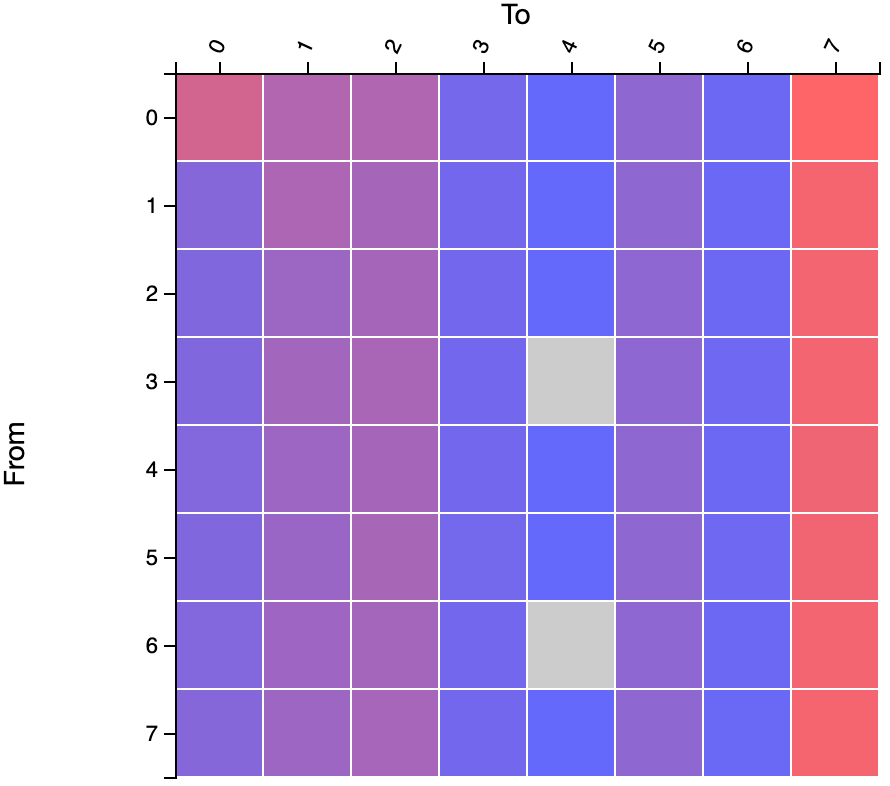
\includegraphics[width=\linewidth]{Paper/images/sumeuler/divconq_static.png}\par
    \caption{Generation 1 objects}
    \label{fig:dnc_gen1}
    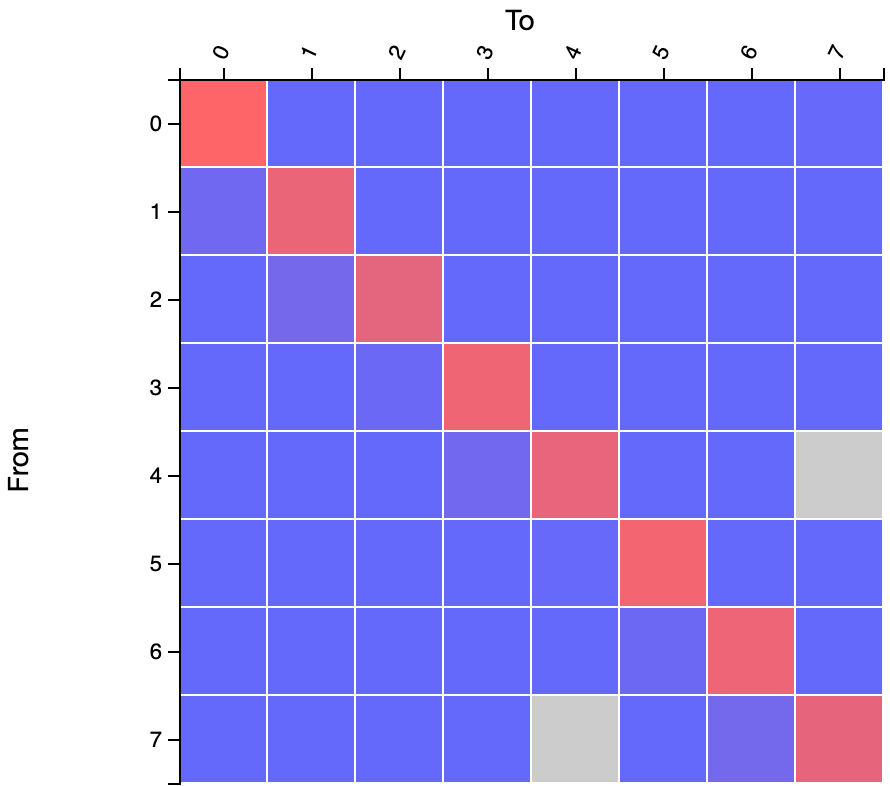
\includegraphics[width=\linewidth]{Paper/images/sumeuler/divconq_gen1.png}\par
    \caption{Generation 2 objects}
    \label{fig:dnc_gen2}
    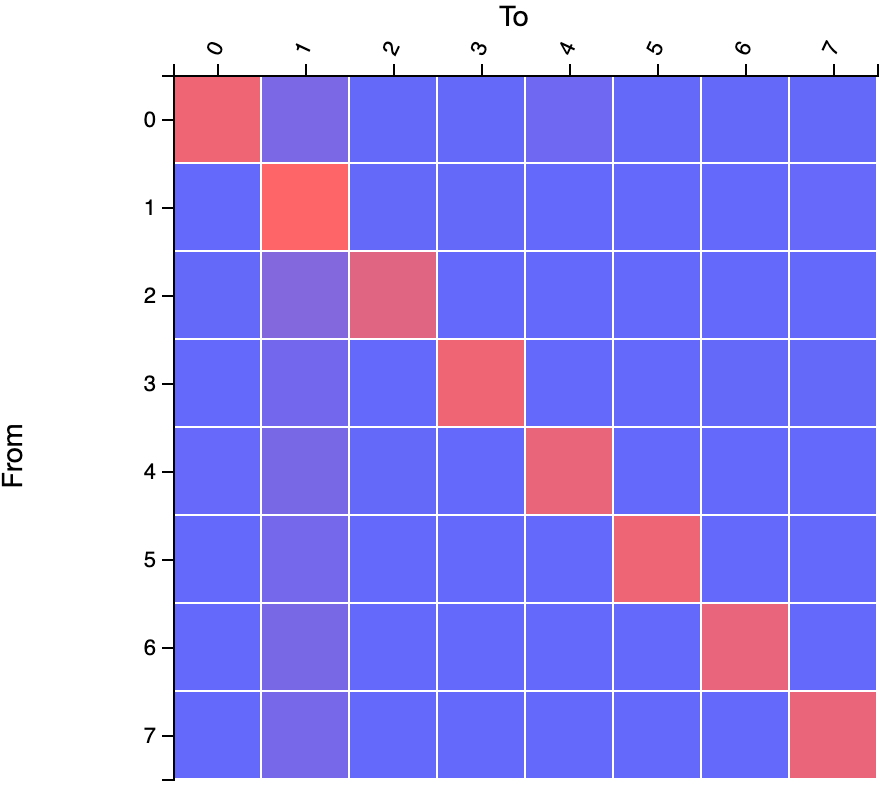
\includegraphics[width=\linewidth]{Paper/images/sumeuler/divconq_gen2.png}\par
    \end{multicols}{3}
    \caption{DNC \lstinline{sumeuler} GC thread locality. Measured by extensions to GHC GC.}
    \label{fig:dnc_static}
\end{figure*}

\begin{figure*}[!htb]
    \centering
    \begin{multicols}{3}
    \caption{Static objects}
    \label{fig:dpp_static}
    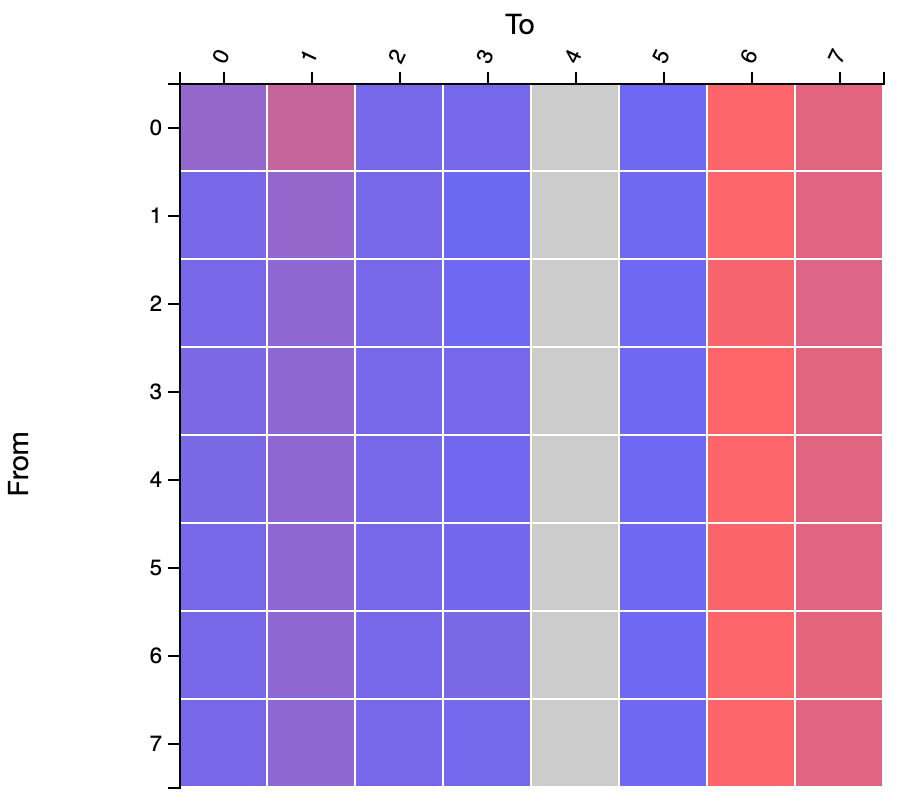
\includegraphics[width=\linewidth]{Paper/images/sumeuler/dp_static.png}\par
    \caption{Generation 1 objects}
    \label{fig:dp_gen1}
    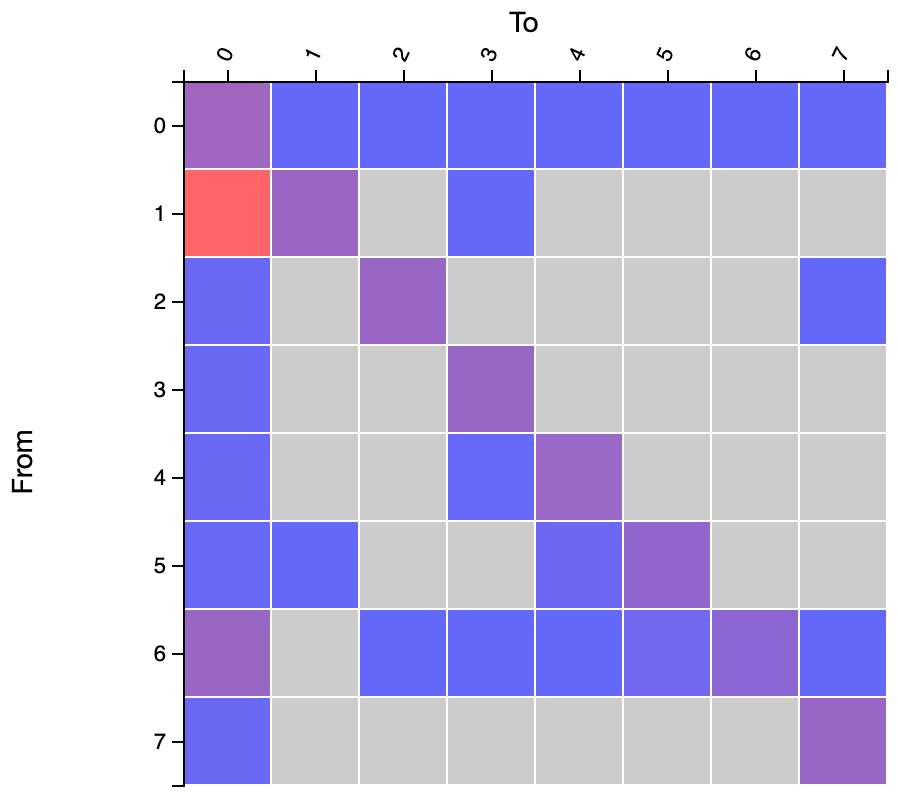
\includegraphics[width=\linewidth]{Paper/images/sumeuler/dp_gen1.png}\par
    \caption{Generation 2 objects}
    \label{fig:dp_gen2}
    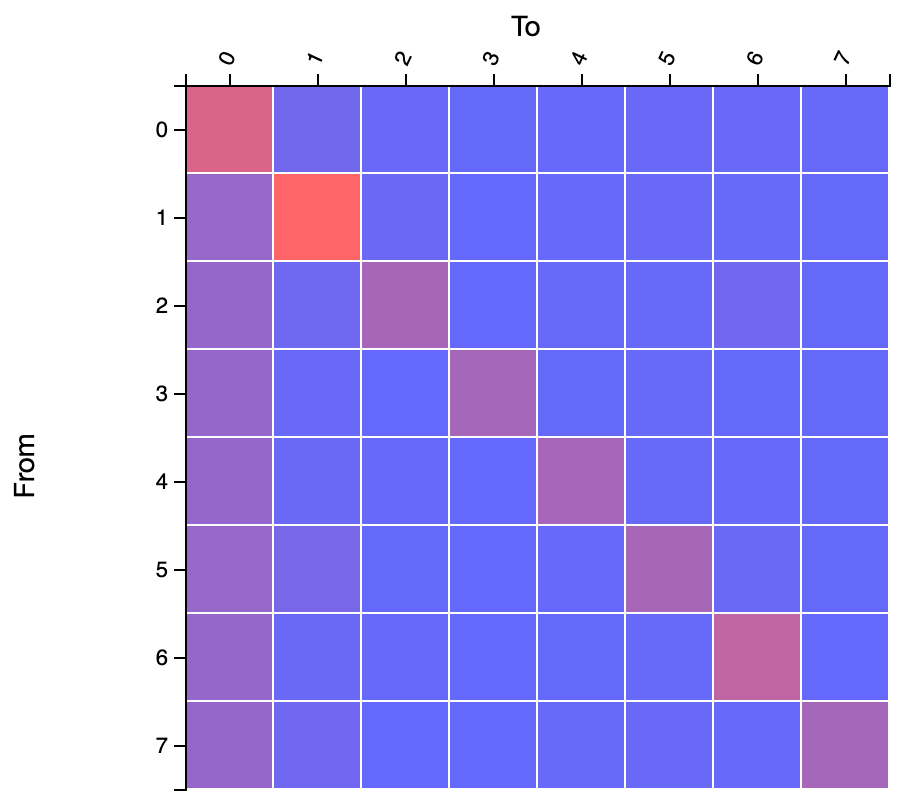
\includegraphics[width=\linewidth]{Paper/images/sumeuler/dp_gen2.png}\par
    \end{multicols}{3}
    \caption{Data parallel \lstinline{sumeuler} GC thread locality. Measured by extensions to GHC GC.}
    \label{fig:dp_static}
\end{figure*}

\begin{figure*}[!htb]
    \centering
    \begin{multicols}{3}
    \caption{Static objects}
    \label{fig:prsaa_static}
    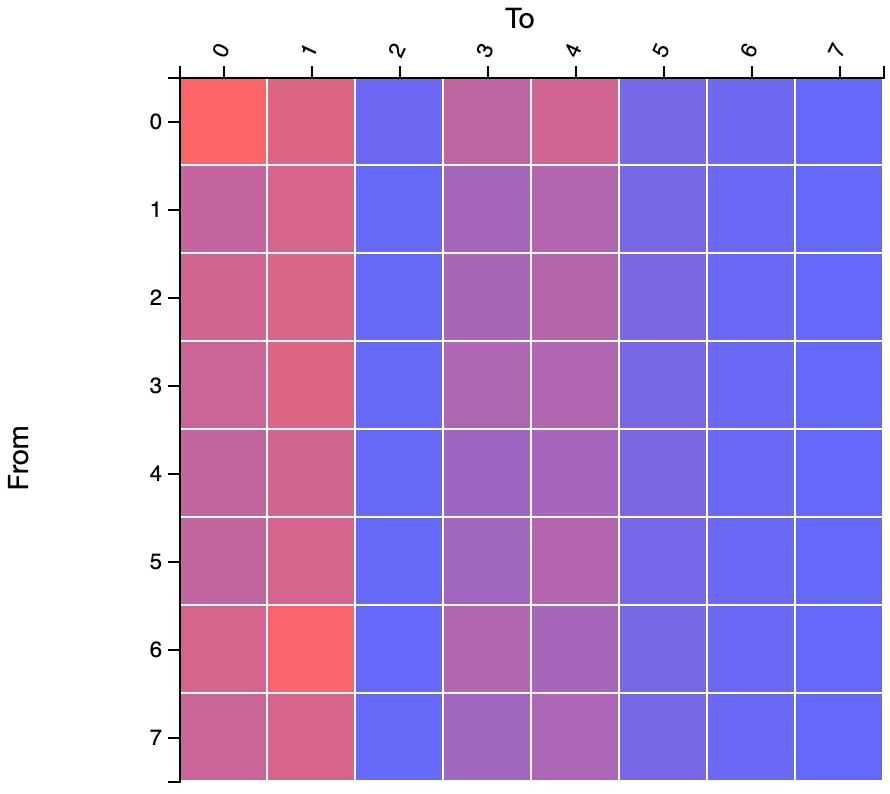
\includegraphics[width=\linewidth]{Paper/images/prsa/prsa_static.png}\par
    \caption{Generation 1 objects}
    \label{fig:prsa_gen1}
    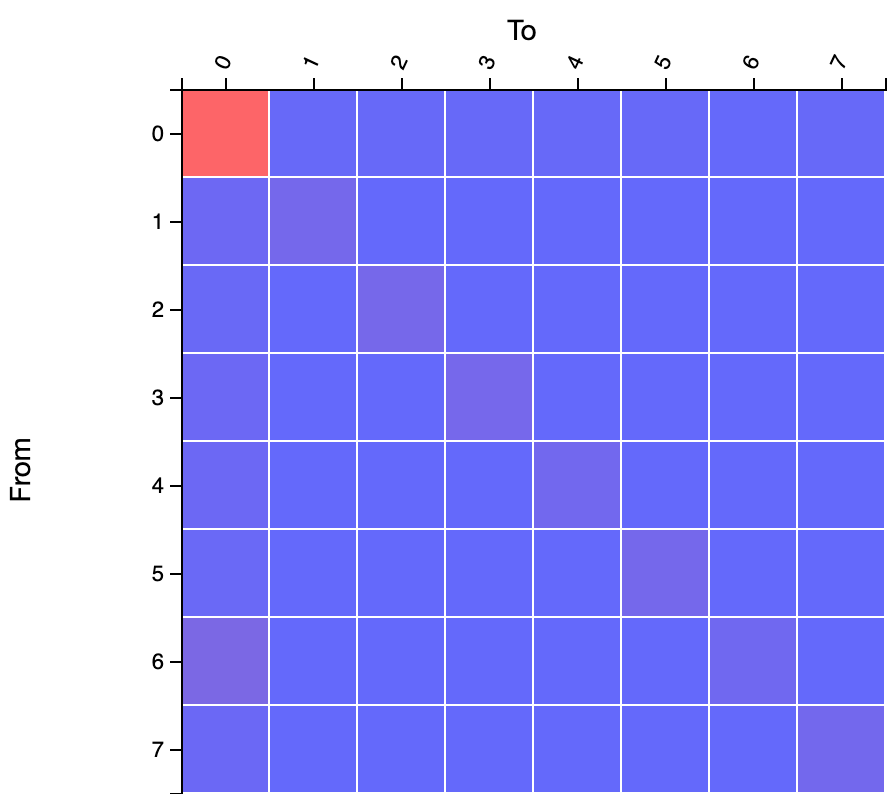
\includegraphics[width=\linewidth]{Paper/images/prsa/prsa_gen1.png}\par
    \caption{Generation 2 objects}
    \label{fig:prsa_gen2}
    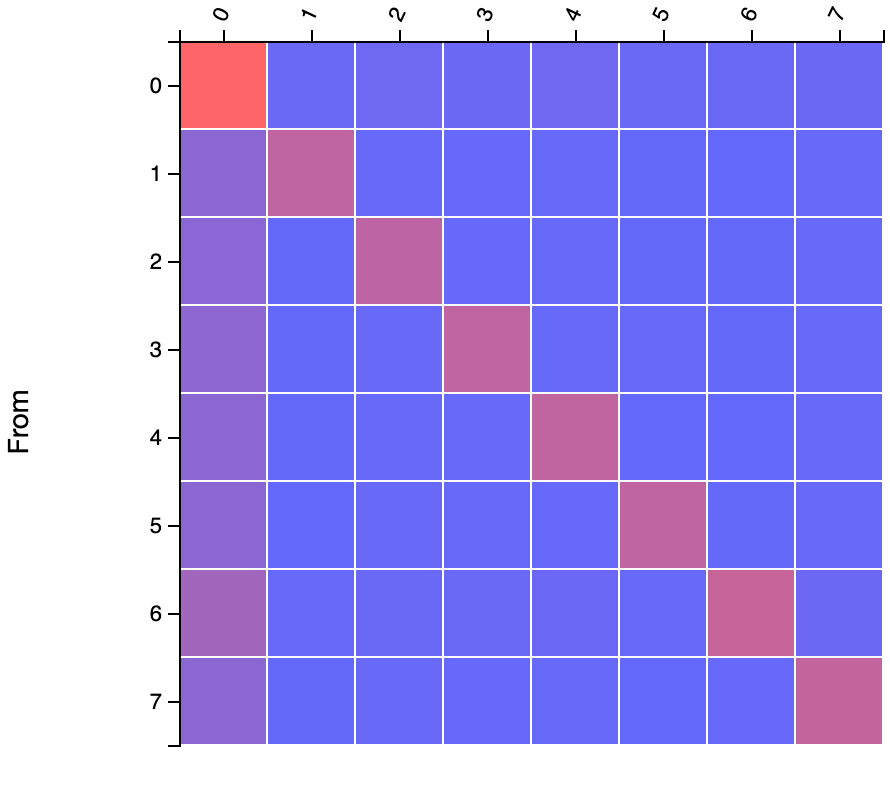
\includegraphics[width=\linewidth]{Paper/images/prsa/prsa_gen2.png}\par
    \end{multicols}{3}
    \caption{\lstinline{prsa} GC thread locality profiles. Measured by extensions to GHC GC.}
    \label{fig:prsa_static}
\end{figure*}


% TODO: GET ALLOCATION RATES FOR ALL GHC HASKELL HEAP PROFILES
%       FINISH COMMENTS ON FIGURE 5
% - - - - - - - - - - - - - - - - - - - - - - - - - - - - - - - - - - - - - - -

\bibliographystyle{abbrv}
\bibliography{paper}

\end{document}
